\documentclass[aspectratio=43,11pt,hyperref={colorlinks=true}]{beamer}
\usetheme{boxes}
\setbeamertemplate{navigation symbols}{}
\definecolor{openstack}{RGB}{149,0,4}
\setbeamercolor{titlelike}{fg=openstack}
\setbeamercolor{structure}{fg=openstack}
\hypersetup{colorlinks,urlcolor=openstack}
\setbeamertemplate{footline}[frame number]
% Inserting graphics
\usepackage{graphicx}
% Side-by-side figures, etc
\usepackage{subfigure}
% Code snippits
\usepackage{listings}
% Color stuff
\usepackage{color}
% for ul
\usepackage{soul}
\usepackage{amsmath}
\usepackage{tikz}
\newcommand\RBox[1]{%
  \tikz\node[draw,rounded corners,align=center,] {#1};%
}
\usepackage{hyperref}
%\usecolortheme{buzz}
%\usecolortheme{wolverine}
%\usetheme{Boadilla}
\usepackage[T1]{fontenc}

\definecolor{mygreen}{rgb}{0,0.6,0}
\definecolor{mygray}{rgb}{0.5,0.5,0.5}
\definecolor{mymauve}{rgb}{0.58,0,0.82}

\lstset{%
  backgroundcolor=\color{white},   % choose the background color; you must add \usepackage{color} or \usepackage{xcolor}
  breakatwhitespace=false,         % sets if automatic breaks should only happen at whitespace
  breaklines=true,                 % sets automatic line breaking
  captionpos=b,                    % sets the caption-position to bottom
  commentstyle=\color{openstack},  % comment style
  extendedchars=true,              % lets you use non-ASCII characters; for 8-bits encodings only, does not work with UTF-8
  keepspaces=true,                 % keeps spaces in text, useful for keeping indentation of code (possibly needs columns=flexible)
  keywordstyle=\color{blue},       % keyword style
%  otherkeywords={*,...},           % if you want to add more keywords to the set
  numbersep=5pt,                   % how far the line-numbers are from the code
  numberstyle=\tiny\color{mygray}, % the style that is used for the line-numbers
  rulecolor=\color{black},         % if not set, the frame-color may be changed on line-breaks within not-black text (e.g. comments (green here))
  showspaces=false,                % show spaces everywhere adding particular underscores; it overrides 'showstringspaces'
  showstringspaces=false,          % underline spaces within strings only
  showtabs=false,                  % show tabs within strings adding particular underscores
  stringstyle=\color{openstack},   % string literal style
}

\setbeamerfont{caption}{series=\normalfont,size=\fontsize{6}{8}}
\setbeamertemplate{caption}{\raggedright\insertcaption\par}

\setlength{\abovecaptionskip}{0pt}
\setlength{\floatsep}{0pt}

\author[Matthew Treinish & Masayuki Igawa]{%
    \texorpdfstring{%
        \begin{columns}
            \column{.45\linewidth}
            \centering
            Matthew Treinish\\
            \href{mailto:mtreinish@kortar.org}{mtreinish@kortar.org}\\
        \texttt{mtreinish on Freenode}
        \column{.45\linewidth}
            \centering
            Masayuki Igawa\\
            \href{mailto:masayuki.igawa@gmail.com}{masayuki.igawa@gmail.com}\\
            \texttt{masayukig on Freenode}
        \end{columns}
        }
    {Matthew Treinish & Masayuki Igawa}
}
\date{July 13, 2016}

\title[Better Testing Through Statistics
\hspace{2em}\insertframenumber/\inserttotalframenumber]{Better Testing Through Statistics}

\begin{document}

{%
\setbeamertemplate{background canvas}{
\includegraphics[width=\paperwidth,height=\paperheight]{background_title.png}}
\setbeamertemplate{footline}{}
\begin{frame}[noframenumbering]
    \setbeamercolor{titlelike}{fg=white}
    \setbeamercolor{structure}{fg=white}
    \setbeamercolor{normal text}{fg=white}
    \hypersetup{colorlinks,urlcolor=white}
    \setbeamercolor{author}{fg=white}
    \setbeamercolor{date}{fg=white}
    \setbeamercolor{background}{bg=openstack}
    \titlepage{}
    \centering
    \href{https://github.com/masayukig/better-testing-through-statistics}{https://github.com/masayukig/better-testing-through-statistics}
\end{frame}
}

\section{What is ``the OpenStack''?}
\begin{frame}
  \frametitle{What is ``the OpenStack''?}
  \begin{itemize}
    \item Open Source Cloud Software: Apache License Version 2.0
    \item consists of a lot of projects: \href{http://governance.openstack.org/reference/projects/index.html}{57 projects}
    \item released every 6 month: Latest version is called `Mitaka'
  \end{itemize}
  \begin{center}
    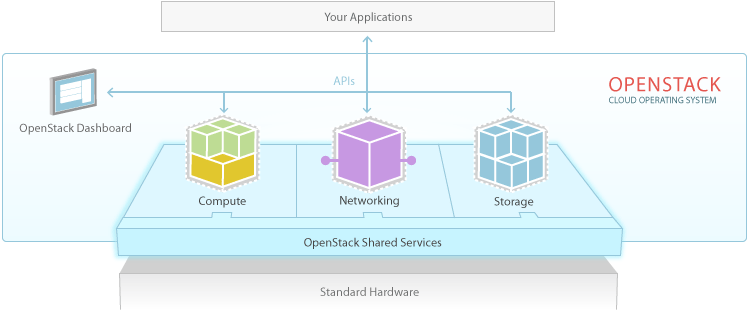
\includegraphics[width=.65\textwidth]{openstack-software-diagram.png}
  \end{center}
\end{frame}

\begin{frame}
  \frametitle{What is ``the OpenStack QA''}
  \begin{itemize}
    \item An official OpenStack project team
    \item \href{https://wiki.openstack.org/wiki/QA}{\ul{Develop, maintain,
      and initiate tools and plans to ensure the upstream stability
      and quality of OpenStack, and its release readiness at any point
      during the release cycle.}}
  \end{itemize}
\end{frame}

\begin{frame}
    \frametitle{Current QA Projects}
    \href{http://governance.openstack.org/reference/projects/quality-assurance.html}{17 repositories (2016/7/8)}
    \begin{columns}
        \column{.45\linewidth}
            \begin{itemize}
                \item{devstack}
                \item{devstack-plugin-cookiecutter}
                \item{devstack-plugin-ceph}
                \item{devstack-vagrant}
                \item{grenade}
                \item{tempest}
                \item{tempest-lib}
                \item{tempest-plugin-cookiecutter}
            \end{itemize}
        \column{.45\linewidth}
            \begin{itemize}
                \item{bashate}
                \item{stackviz}
                \item{hacking}
                \item{eslint-config-openstack}
                \item{os-testr}
                \item{os-performance-tools}
                \item{openstack-health dashboard}
                \item{karma-subunit-reporter}
            \end{itemize}
    \end{columns}
\end{frame}

\section{What is ``the OpenStack Gate''?}
\begin{frame}
    \frametitle{What is ``the OpenStack Gate''?}
	\begin{center}
		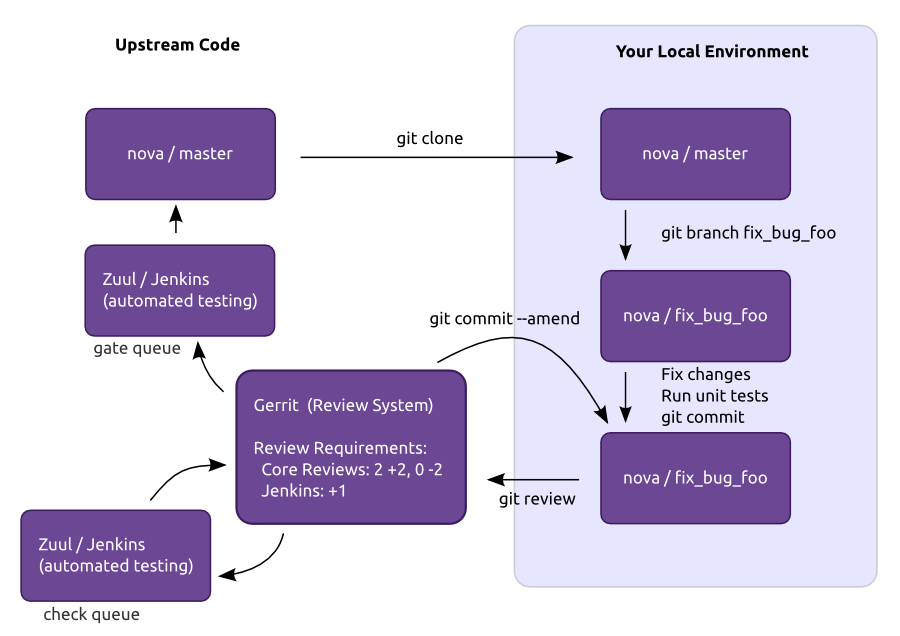
\includegraphics[width=.65\textwidth]{code_review.png}
	\end{center}
\end{frame}

\begin{frame}
\frametitle{What Happens when you push a change?}
\begin{center}
	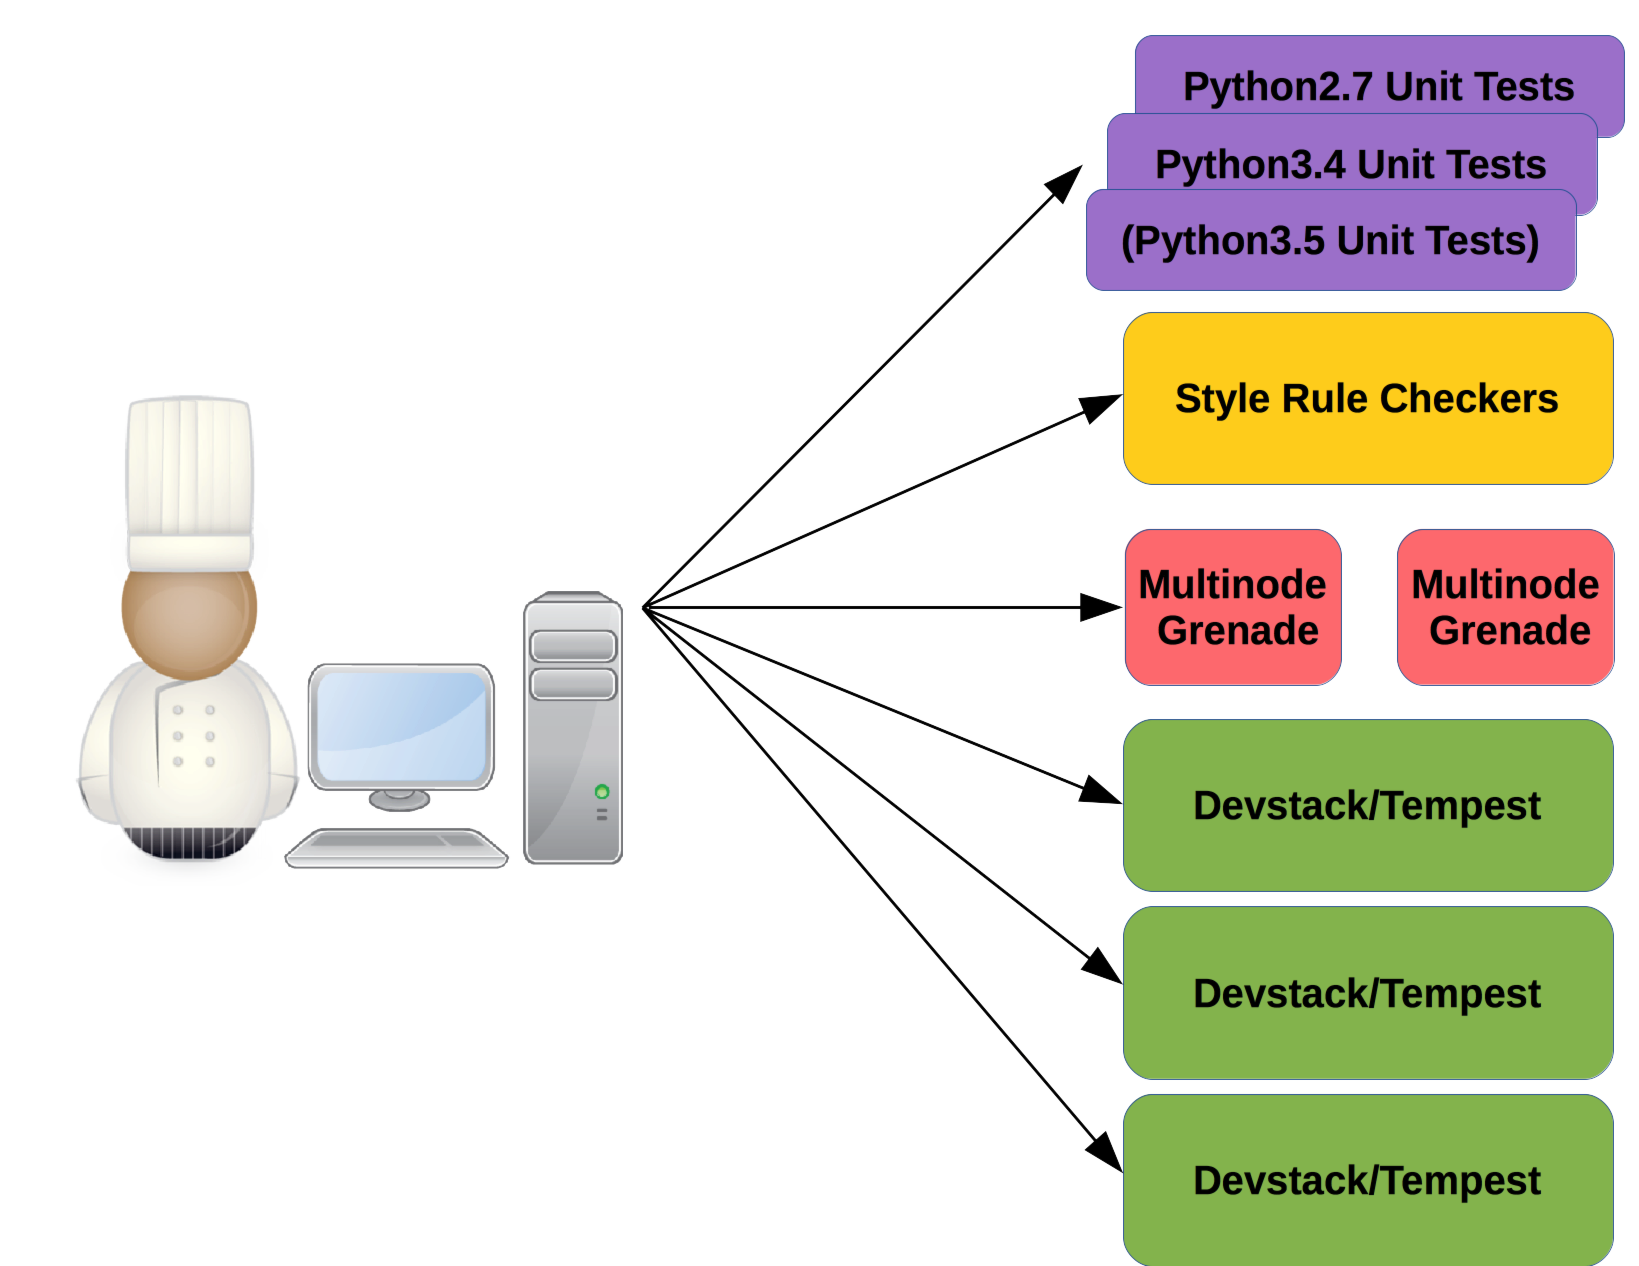
\includegraphics[width=.7\textwidth]{jobs.png}
\end{center}
\end{frame}

\begin{frame}
\begin{center}
    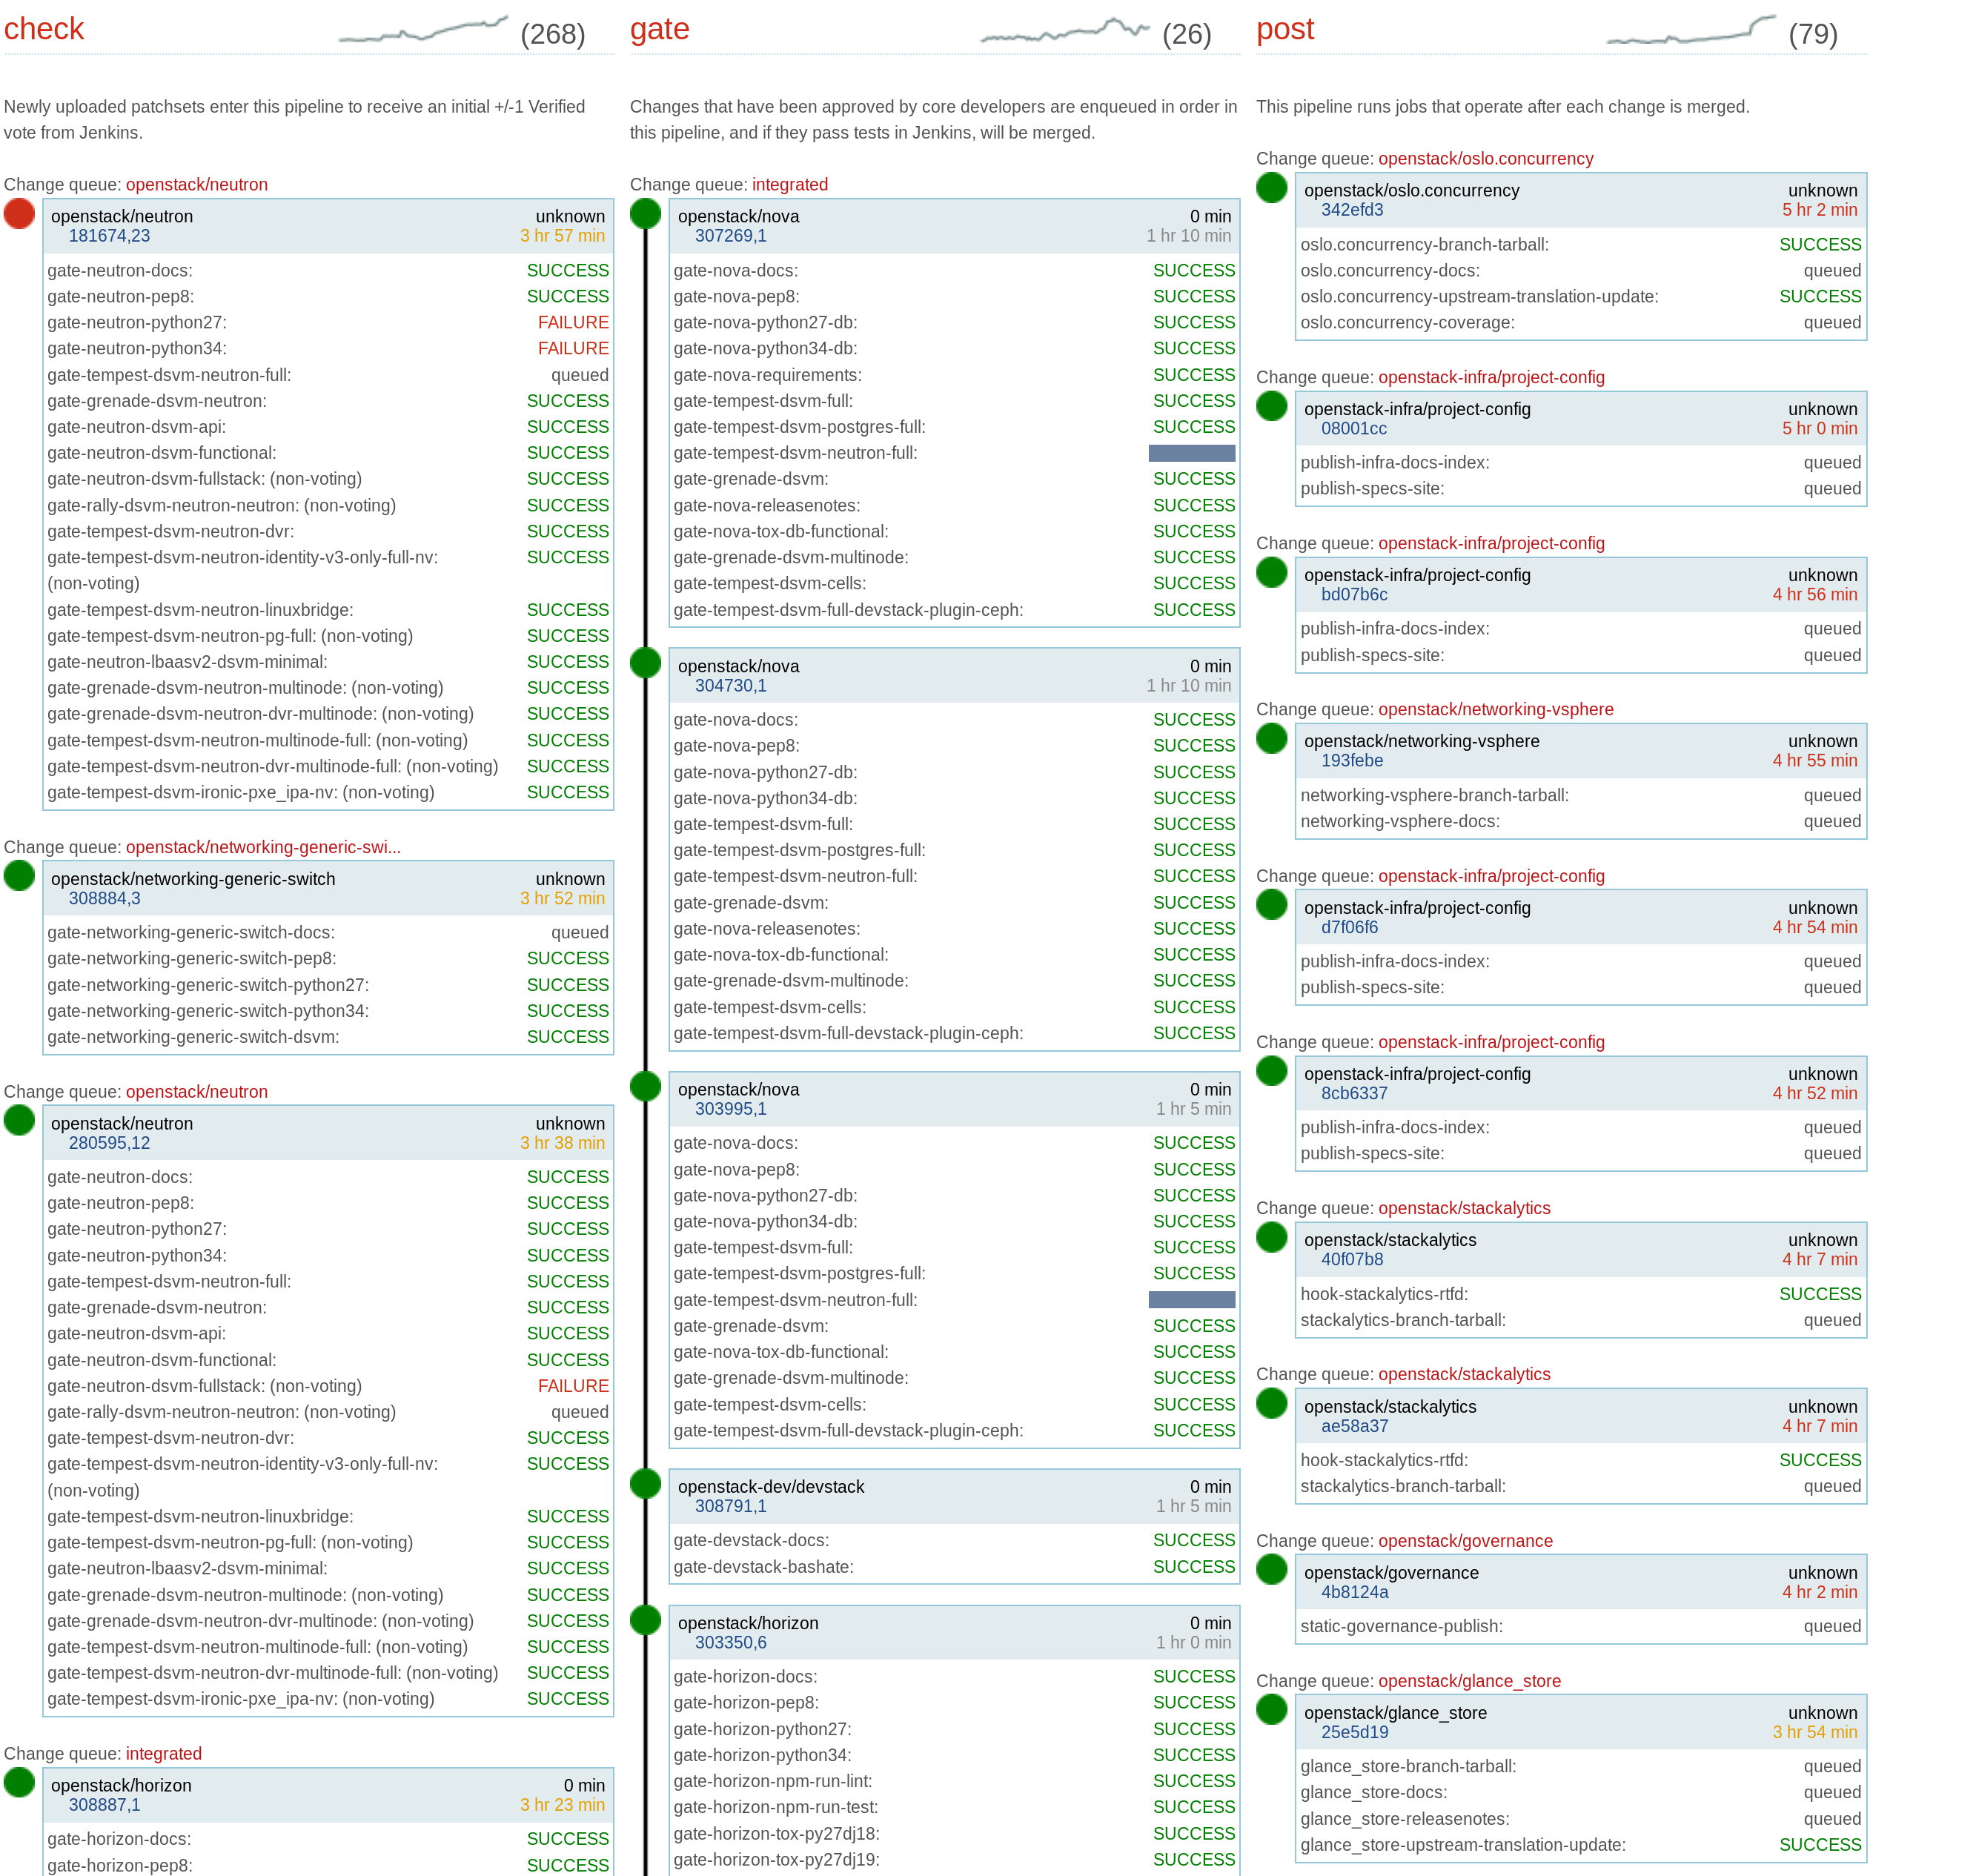
\includegraphics[width=.8\textwidth]{ZuulStatus.png}
\end{center}
\end{frame}

\begin{frame}
\frametitle{The Size of the Gate}
  \begin{columns}[T]
    \begin{column}{.48\textwidth}
      \textbf{One Proposed Change Generates:}
      \begin{itemize}
        \item 5--25 Devstacks
        \item \textasciitilde10,000 integration tests (roughly 1.5k per devstack)
        \item \textasciitilde151 2nd level guests created in each devstack cloud
        \item \textasciitilde1 GB of logs uncompressed for each run
      \end{itemize}
      \textbf{In aggregate:}
      \begin{itemize}
        \item \textasciitilde12,500 jobs run in check and gate daily
        \item \textasciitilde0.01\% individual tempest test failure rate
        \item \textasciitilde.77\% tempest run failure rate
      \end{itemize}
    \end{column}
    \begin{column}{.48\textwidth}
      \centering
      \textbf{Number of Tempest Tests per Day in the Gate Queue:}
      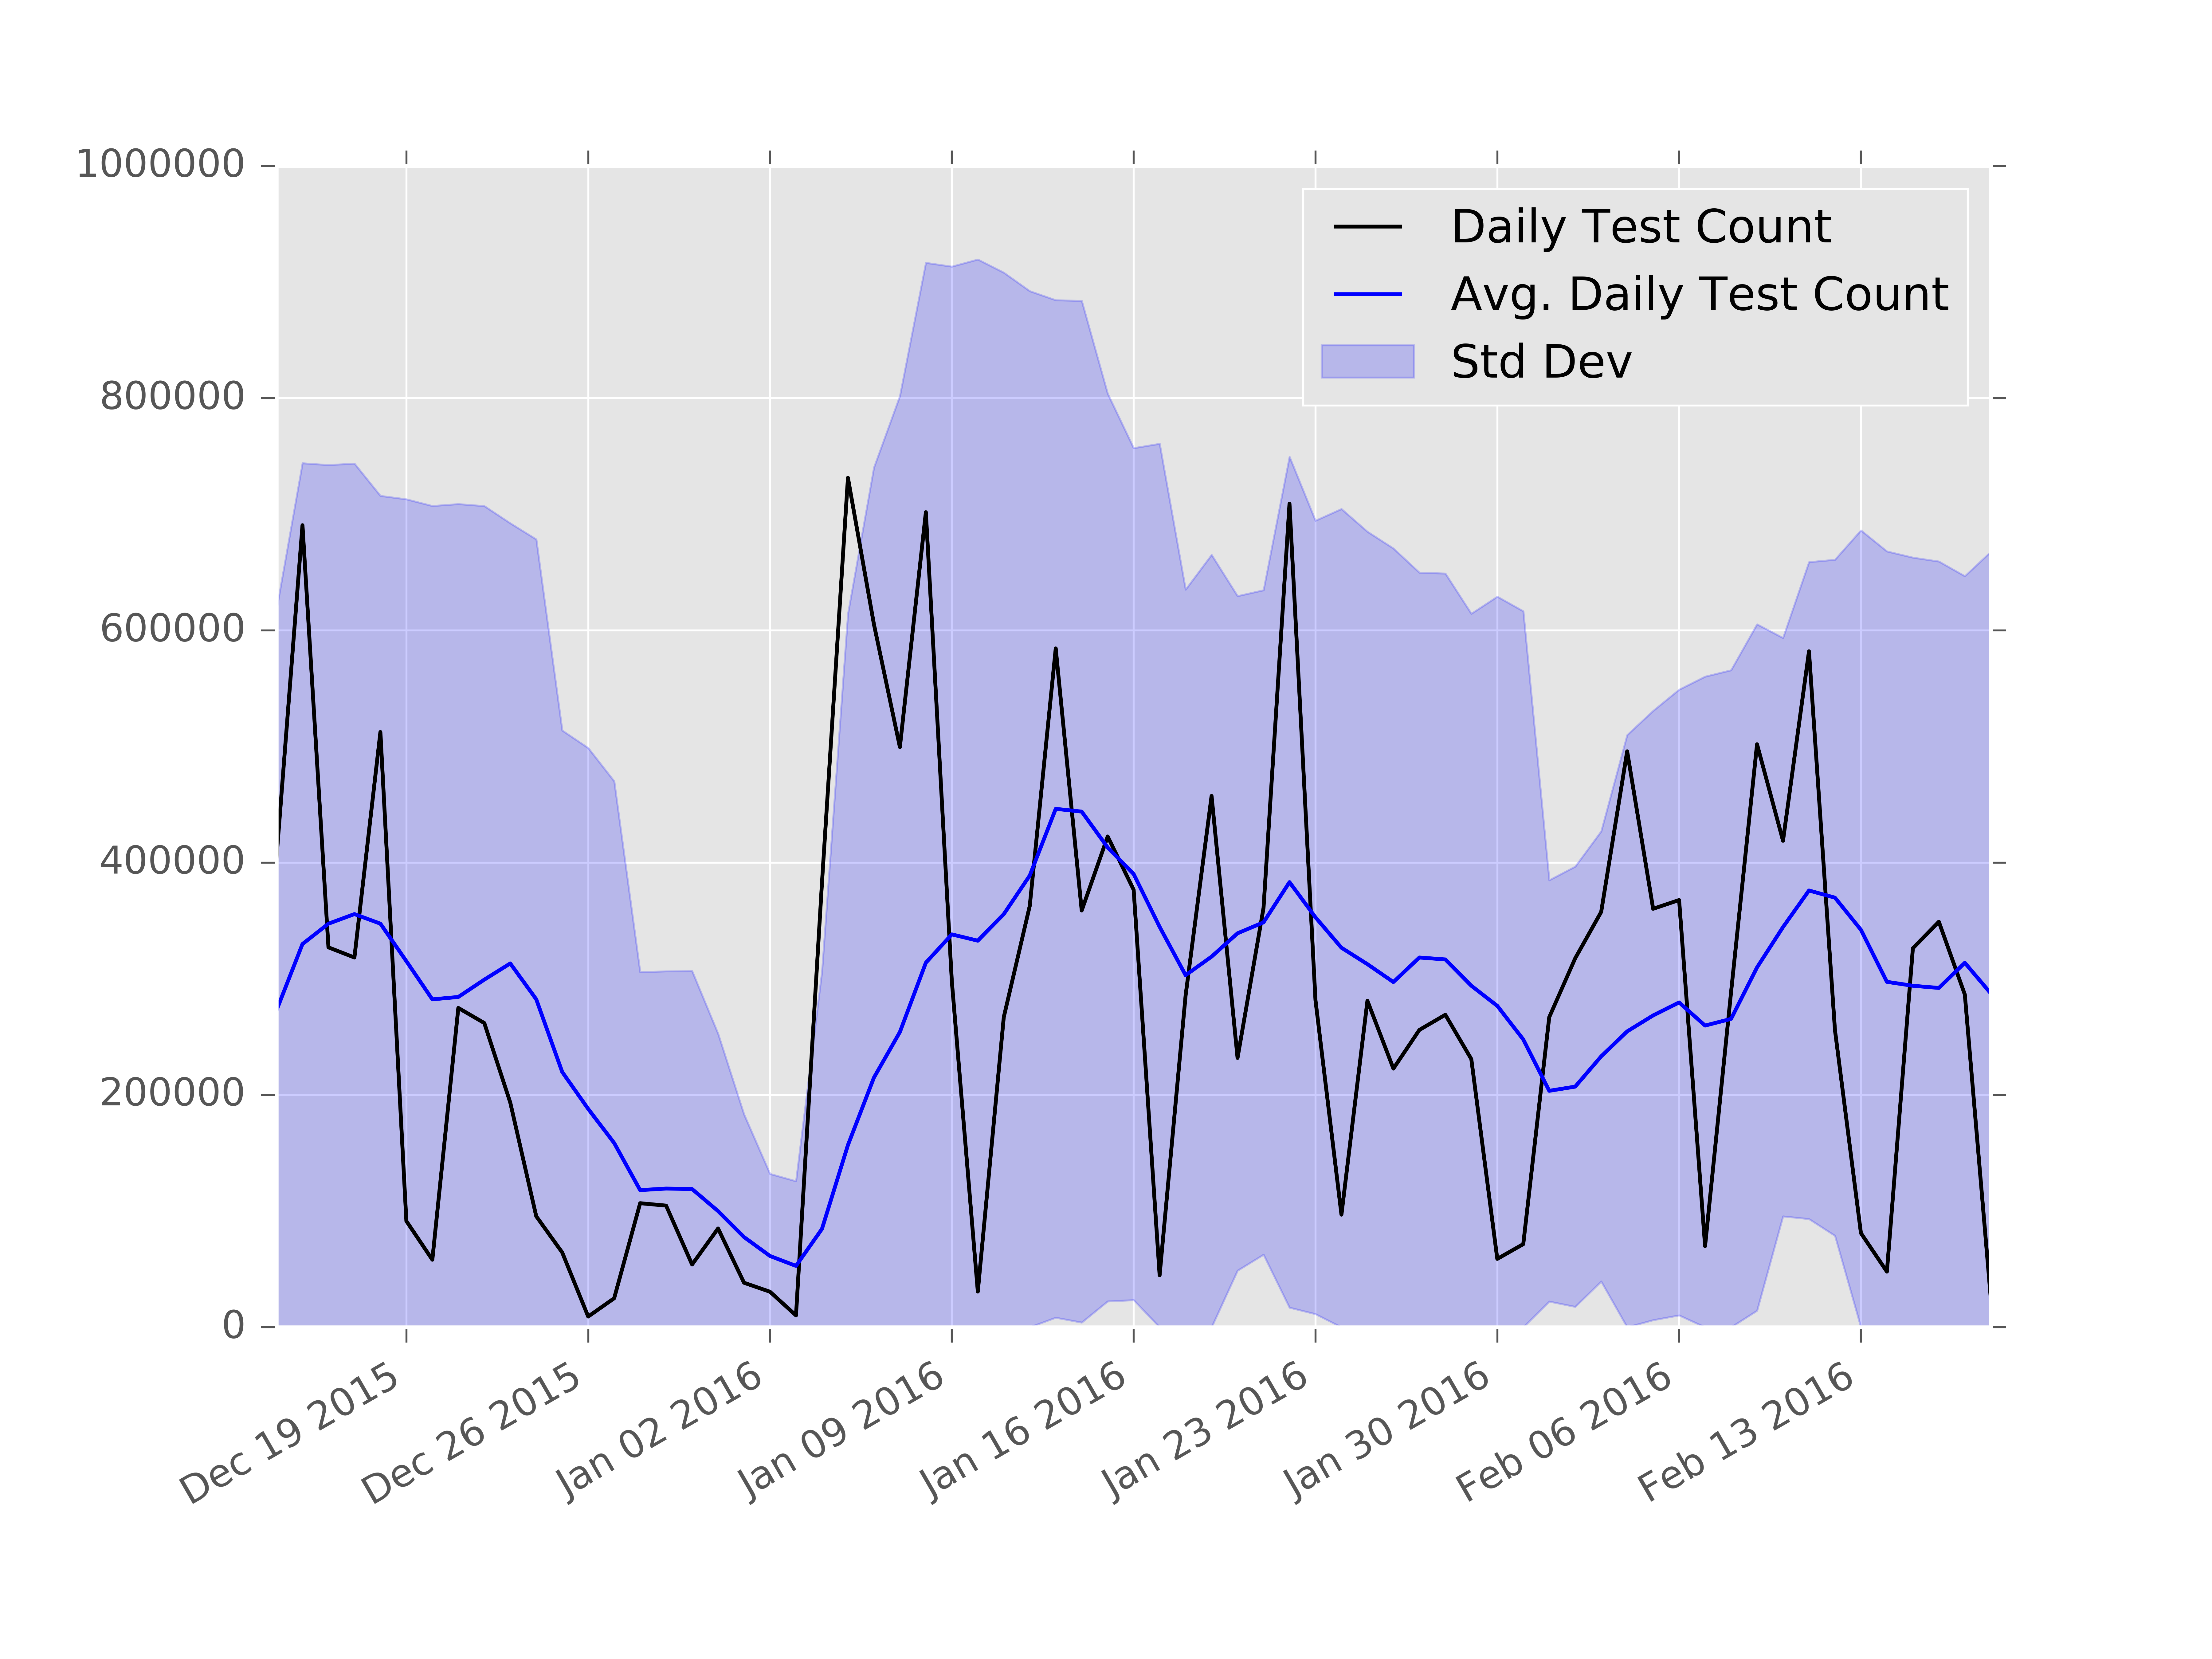
\includegraphics[width=1.22\textwidth]{tempest-gate-count.png}
    \end{column}
  \end{columns}
\end{frame}

\subsection{Examples of Complications with the Size}
\begin{frame}
  \frametitle{Log Server}
  \begin{itemize}
    \item Log Server: \href{http://logs.openstack.org/}{http://logs.openstack.org/}
    \item Archive of all artifacts from all jobs for \textasciitilde4 months
%http://cacti.openstack.org/cacti/graph.php?action=view&local_graph_id=717&rra_id=all
    \item \textasciitilde8 TB of data compressed
  \end{itemize}
  \begin{center}
    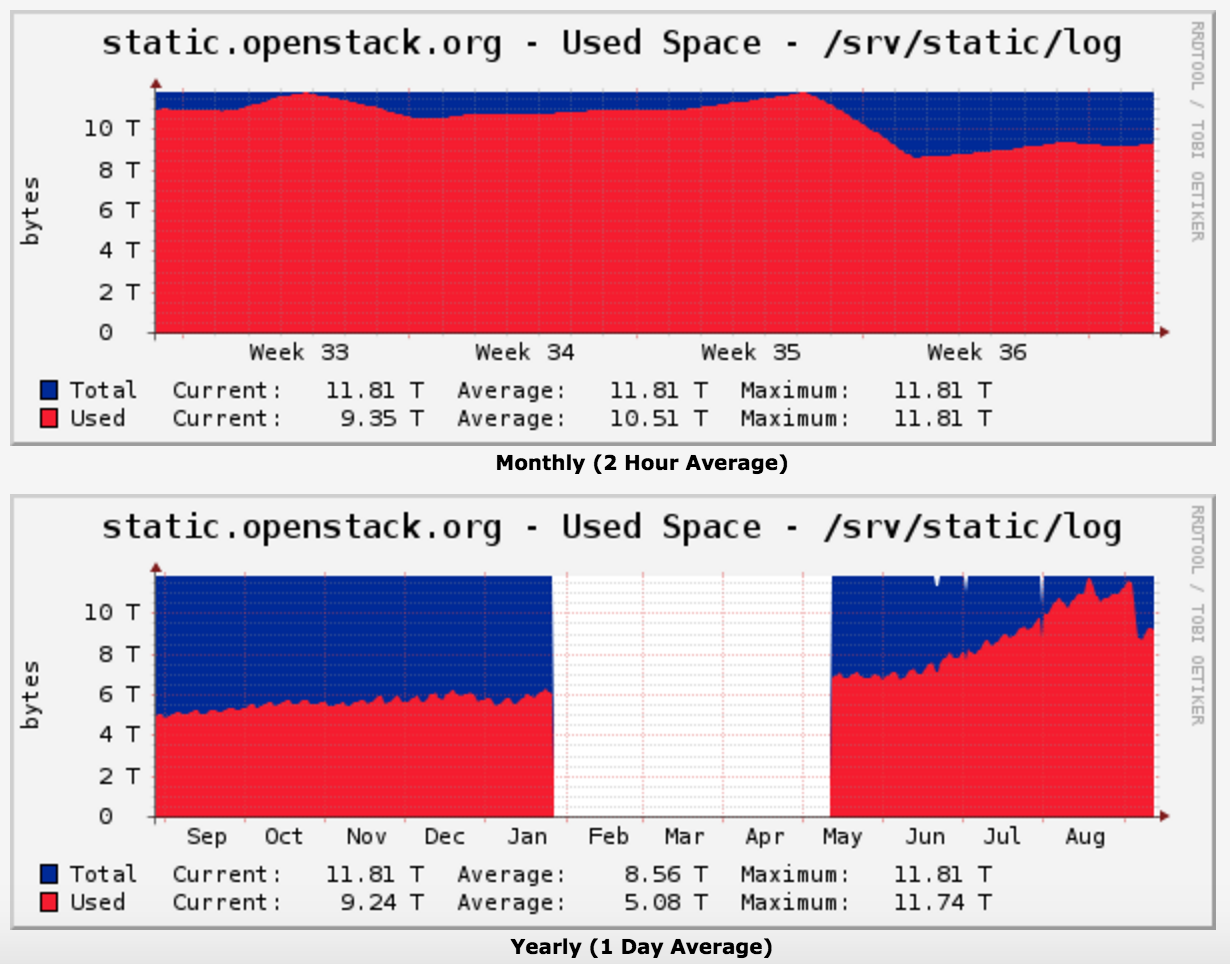
\includegraphics[width=.55\textwidth]{cacti-static-openstack-org-log-graph.png}
  \end{center}
\end{frame}

\begin{frame}
  \frametitle{Problem/Issue}
  \begin{itemize}
    \item It's difficult to find a problem from the large amount of log
    \item It's difficult to find performance regression/improvement
    \item
  \end{itemize}
\end{frame}

\section{Solutions}
\begin{frame}
  \frametitle{General Approach}
    \begin{itemize}
        \item Look at things on the larger scale
        \item Use statistics and data mining to find
        \item Make the data from test runs open and accesible to
        \item Ensure there are APIs for accessing everything
    \end{itemize}
\end{frame}

\begin{frame}
  \frametitle{Graphite}
  \begin{itemize}
    \item \href{http://graphite.openstack.org/}{http://graphite.openstack.org/}
    \item Infra services report to graphite
    \item Include job results
    \item Limited to job level data
    \item Time based, can't be linked to an individual job
    \item
  \end{itemize}
  \begin{center}
    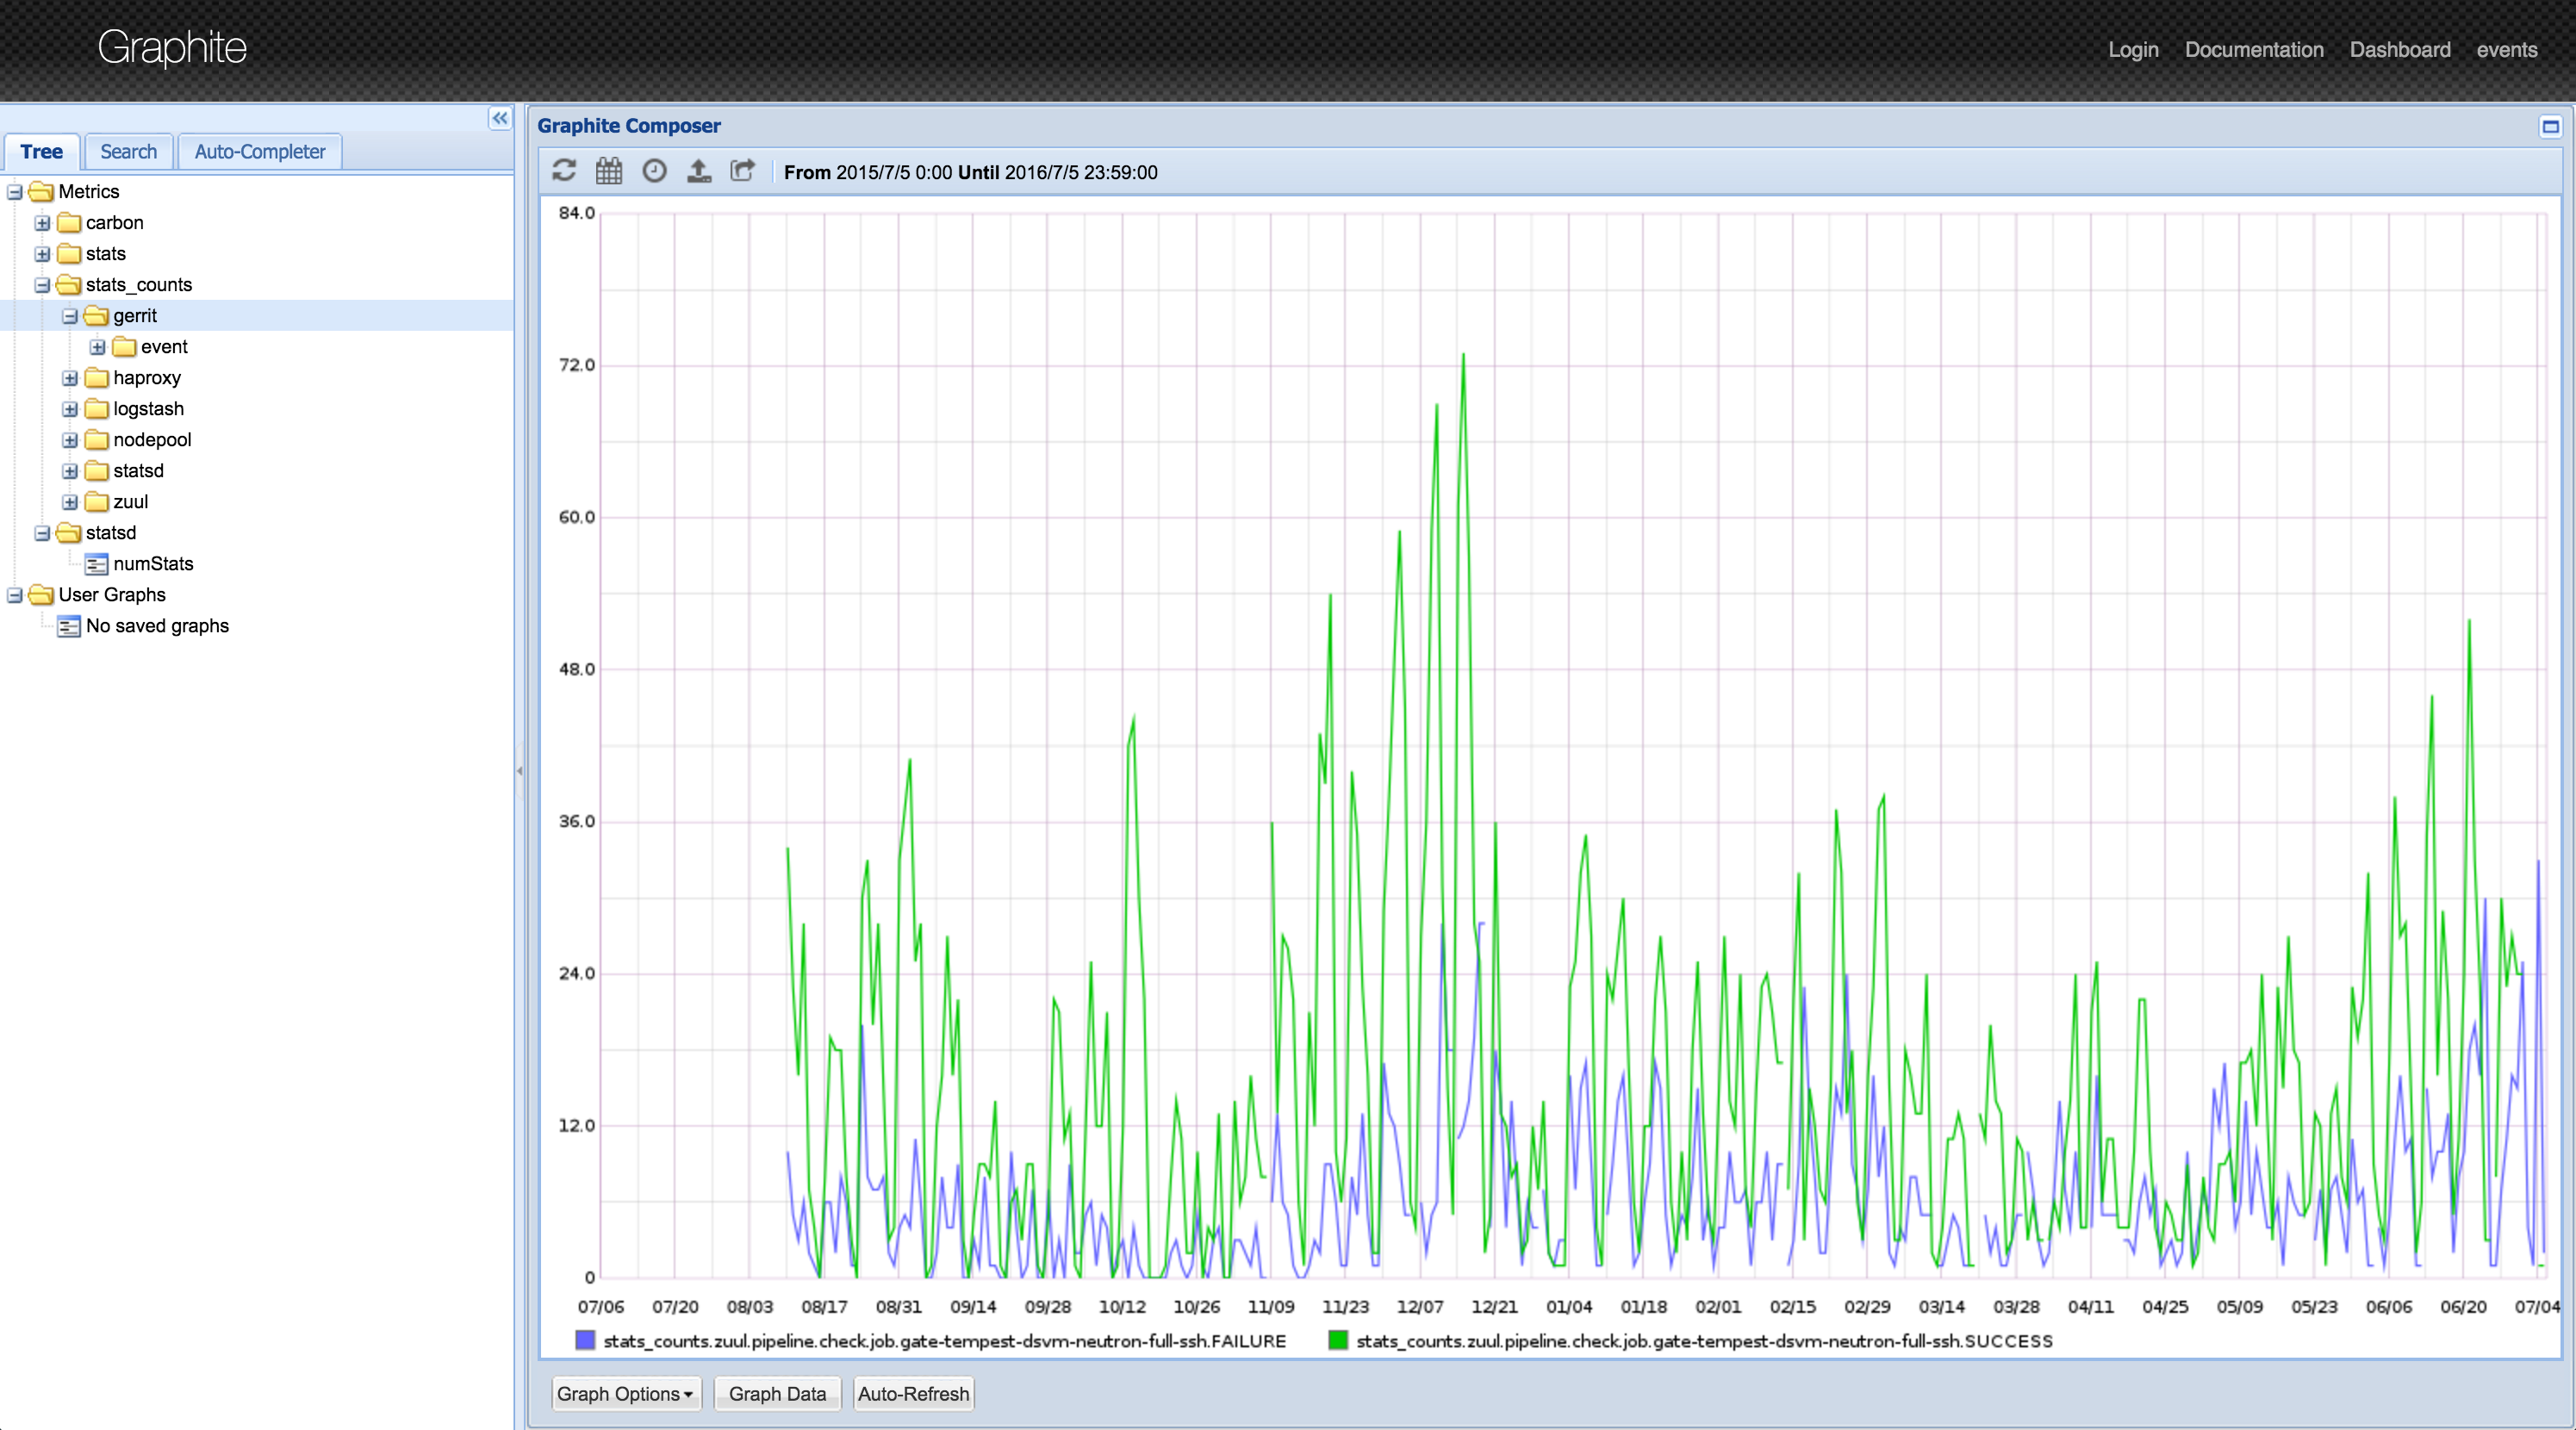
\includegraphics[width=.65\textwidth]{graphite-sample.png}
  \end{center}
\end{frame}

\begin{frame}
  \frametitle{Grafana}
  \begin{itemize}
    \item \href{http://grafana.openstack.org/}{http://grafana.openstack.org/}
    \item Provides a layer on top of graphite to easily make useful visualizations
    \item Adds a number of dashboards
    \item Some projects using this to track job failure rates
  \end{itemize}
  \begin{center}
    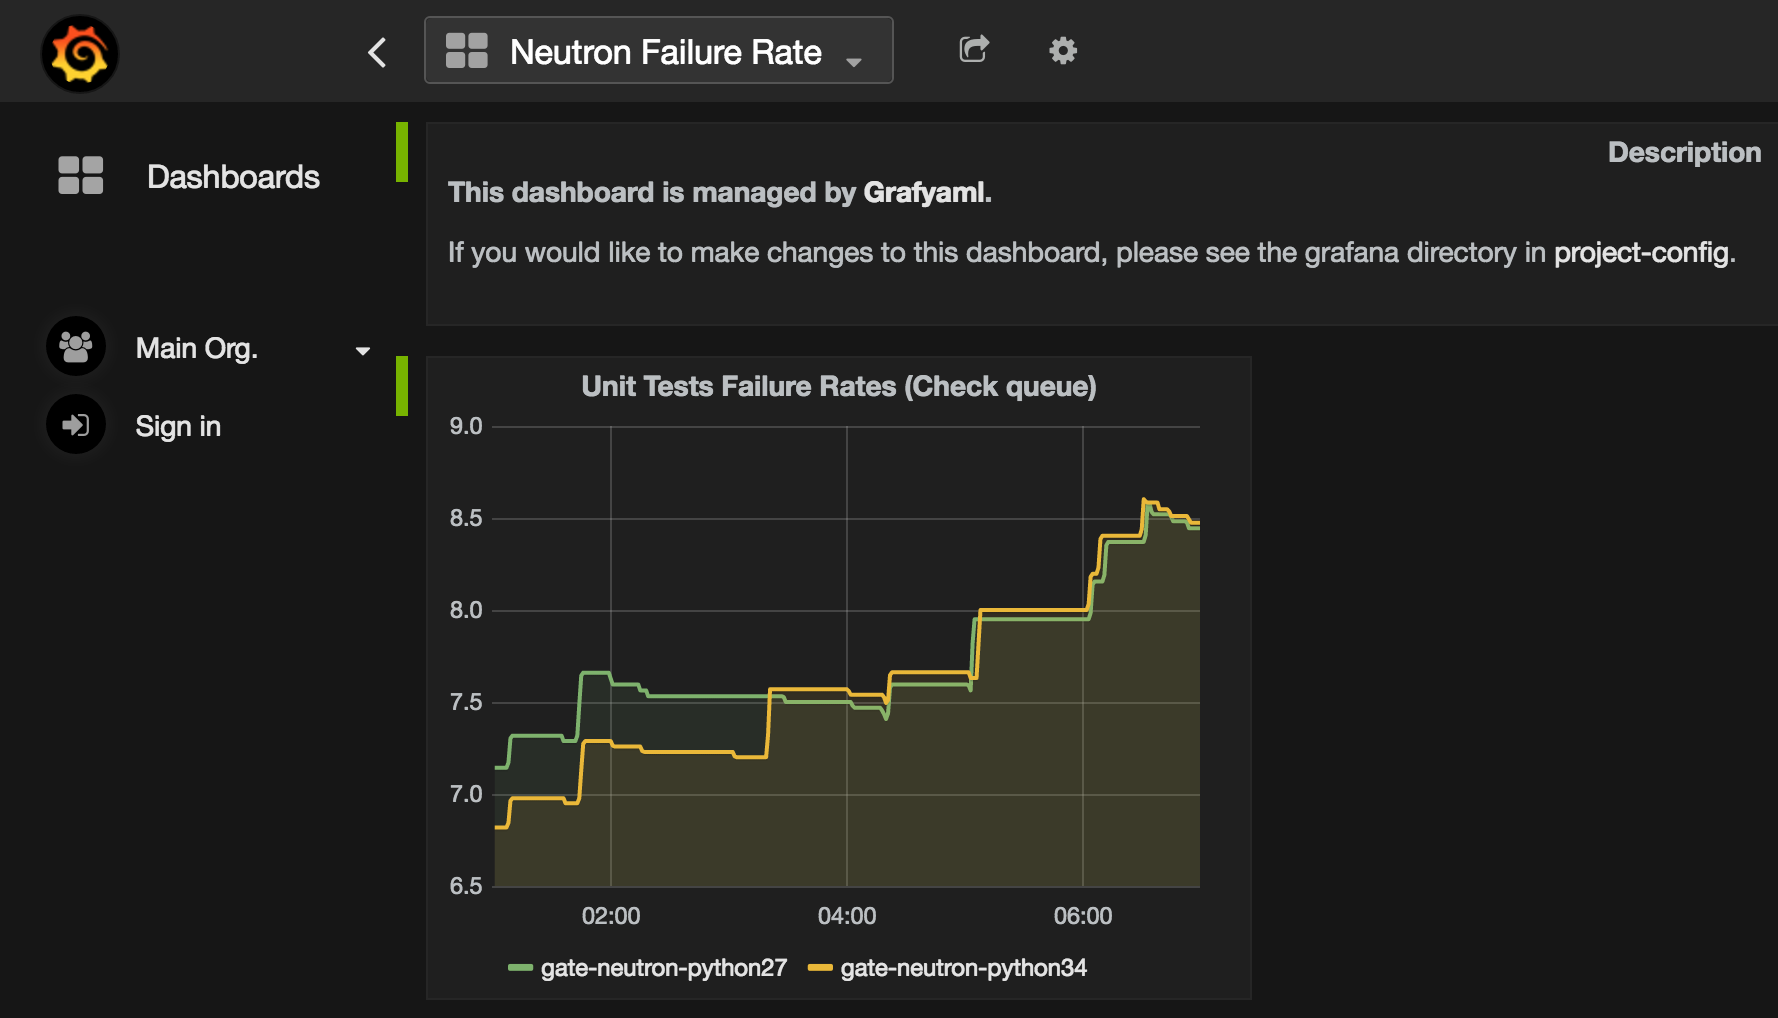
\includegraphics[width=.7\textwidth]{grafana-sample.png}
  \end{center}
\end{frame}

\begin{frame}
  \frametitle{ELK}
  \begin{itemize}
    \item Elasticsearch, Logstash, Kibana
    \item \href{http://logstash.openstack.org}{http://logstash.openstack.org}
    \item Provides a search engine on top of are job artifacts
    \item Limited to 10 days of results
  \end{itemize}
  \begin{center}
    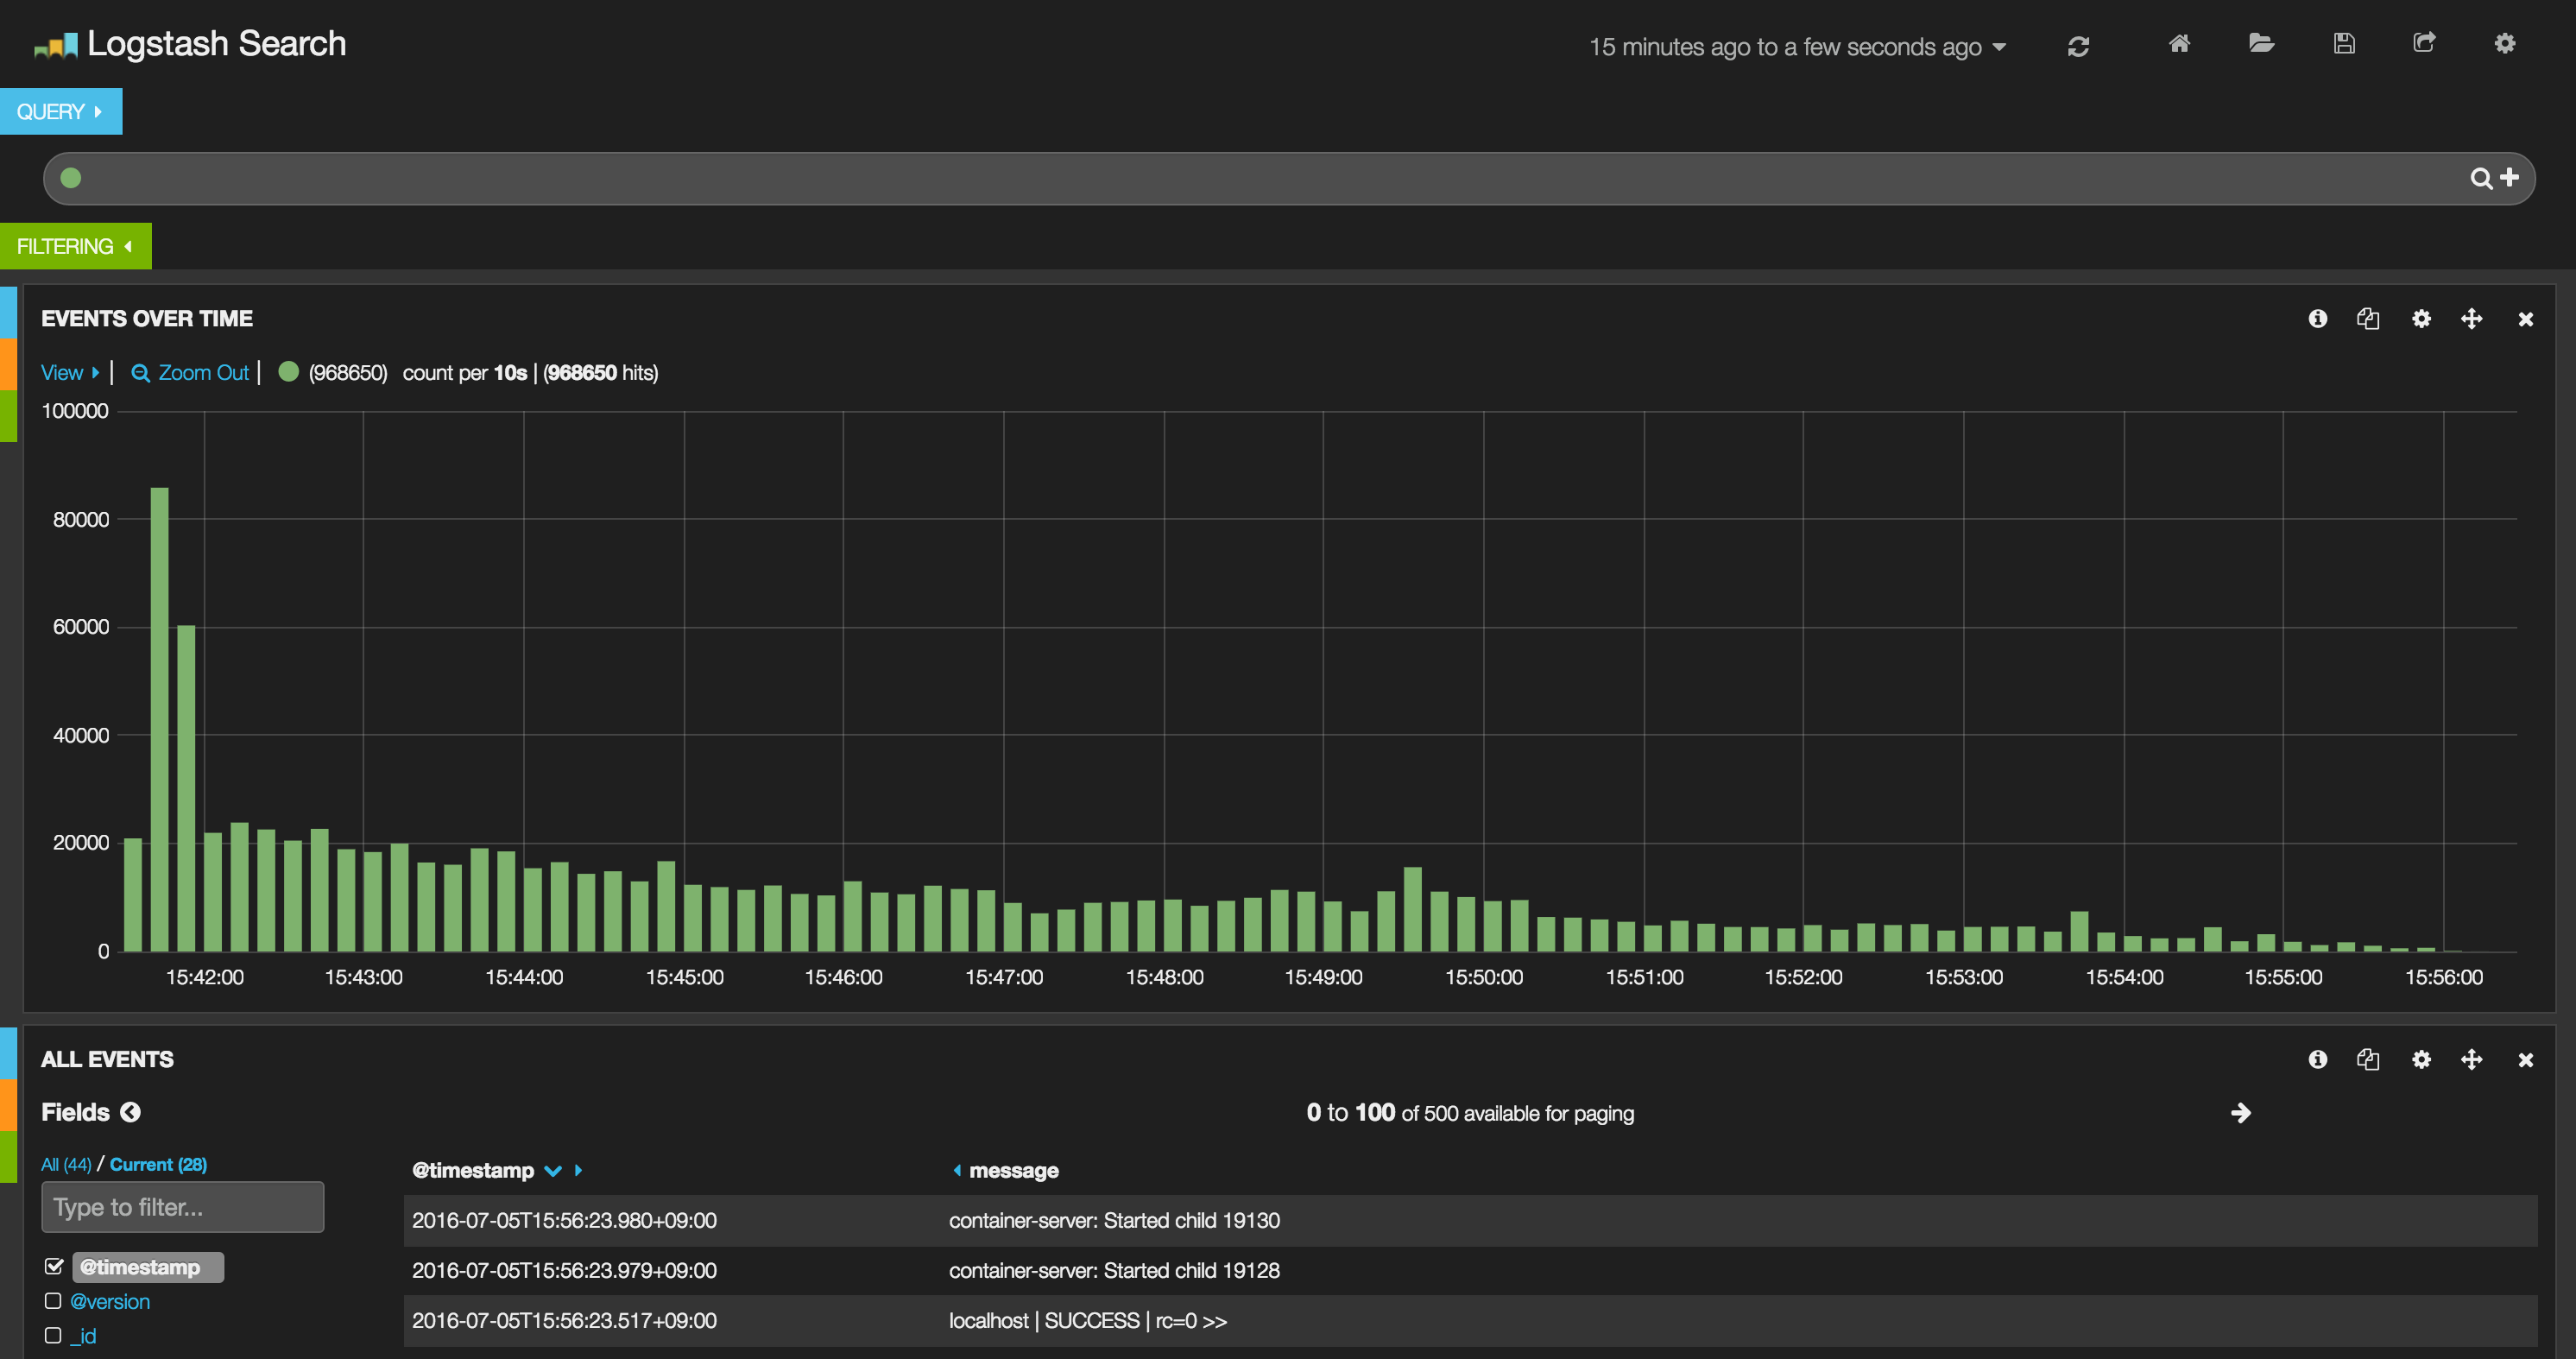
\includegraphics[width=.75\textwidth]{kibana-sample.png}
  \end{center}
\end{frame}

\begin{frame}
  \frametitle{Elastic Recheck}
  \begin{itemize}
    \item Designed to answer the question ``Have you seen this recently?''
    \item \href{http://status.openstack.org/elastic-recheck/}{http://status.openstack.org/elastic-recheck/}
    \item
  \end{itemize}
  \begin{center}
    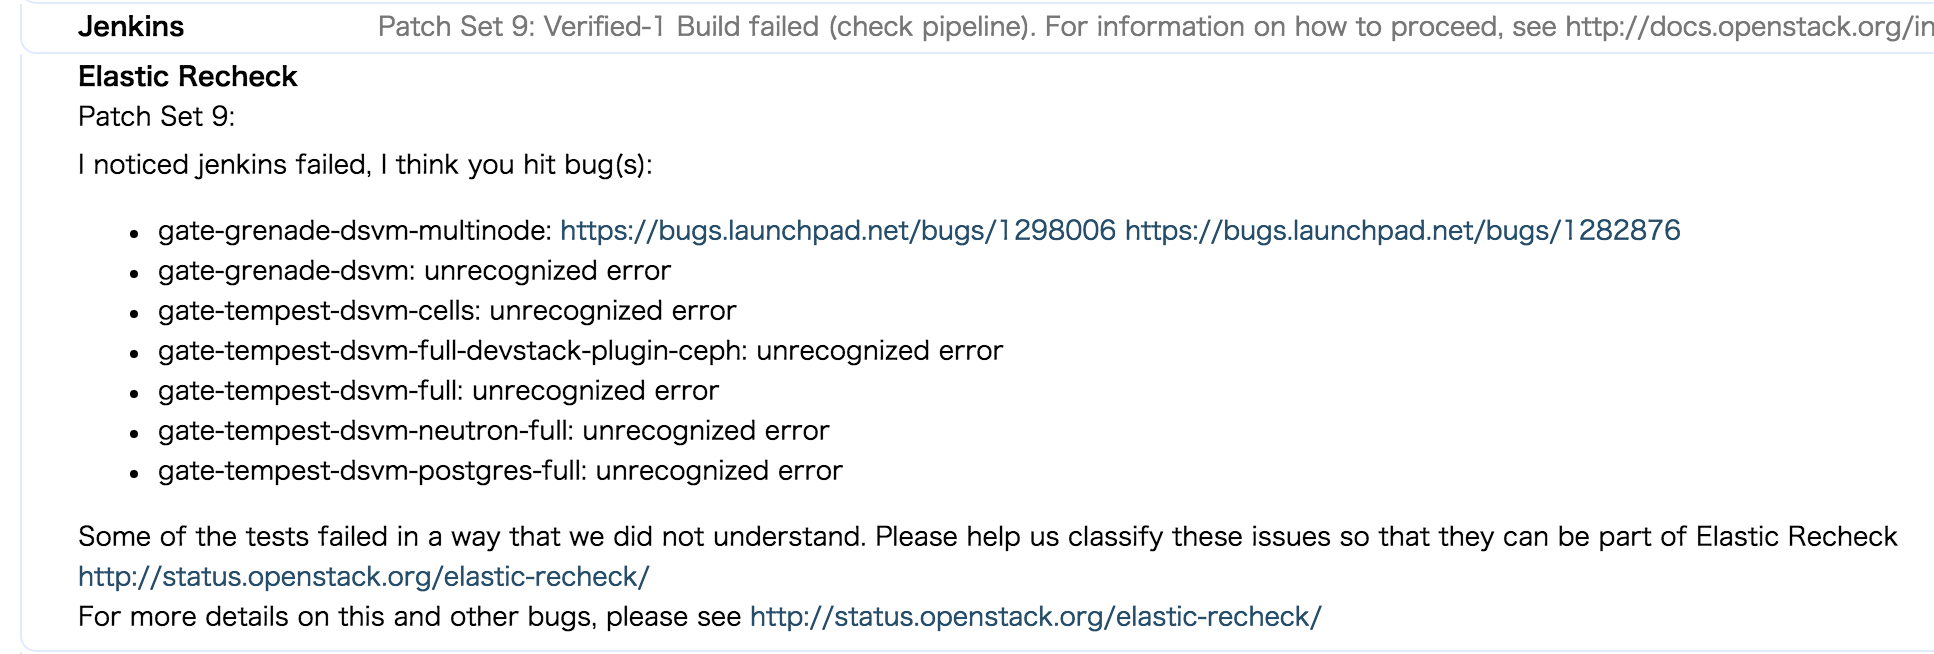
\includegraphics[width=.9\textwidth]{elastic-recheck-sample.png}
  \end{center}
\end{frame}


\begin{frame}
    \frametitle{subunit2sql}
    \begin{itemize}
        \item Designed to store test results data in a sql database
        \item Provides a DB schema and a python API for interacting with the
              database
        \item Used to the results from test runs for 6 months
        \item
    \end{itemize}
\end{frame}

\begin{frame}
    \frametitle{subunit2sql in OpenStack Infrastructure}
    \begin{center}
        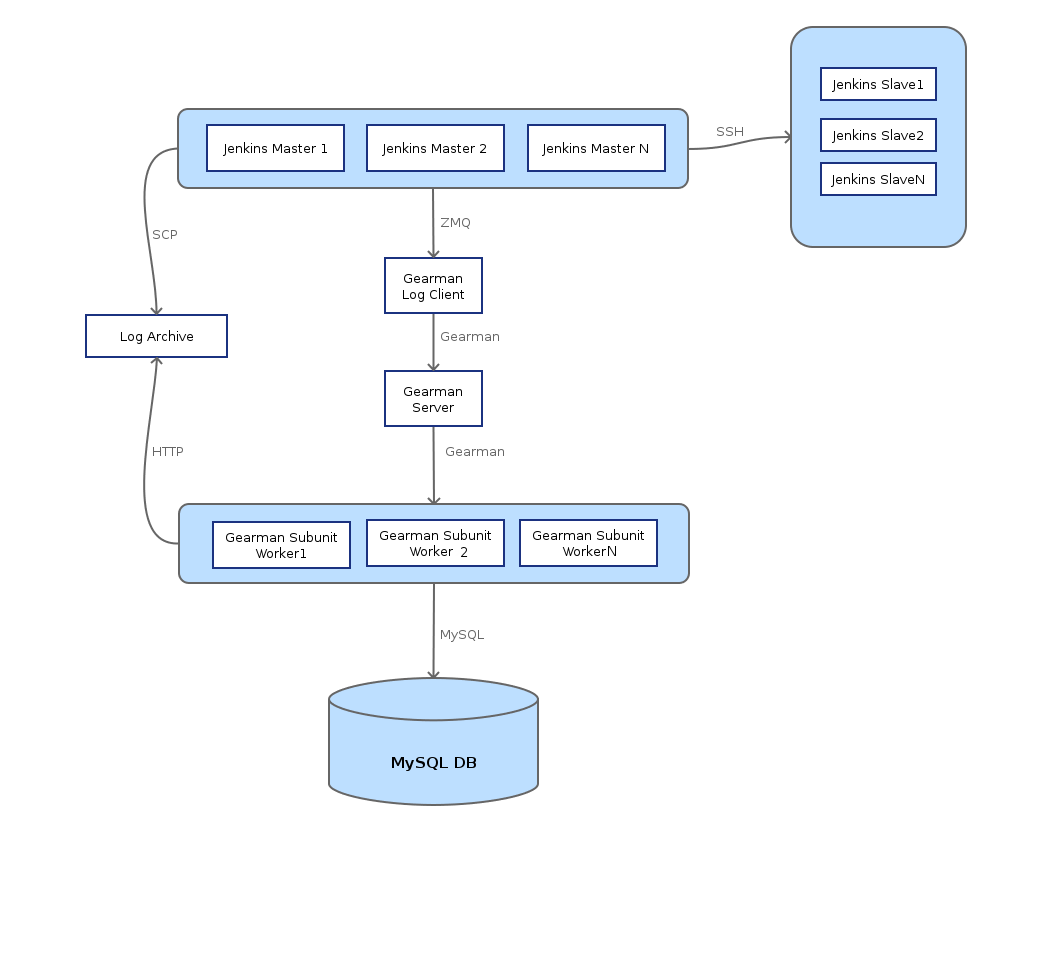
\includegraphics[height=1.1\textheight]{subunit2sql-collection.png}
    \end{center}
\end{frame}

\begin{frame}
    \frametitle{openstack-health}
    \begin{itemize}
        \item \href{http://status.openstack.org/openstack-health/\#/}{http://status.openstack.org/openstack-health/\#/}
        \item Designed to be a single point of access for all the data about the gate
        \item Currently can leverage subunit2sql and elastic-recheck
    \end{itemize}
\end{frame}

\begin{frame}
    \frametitle{OpenStack-Health Architecture}
    \begin{center}
        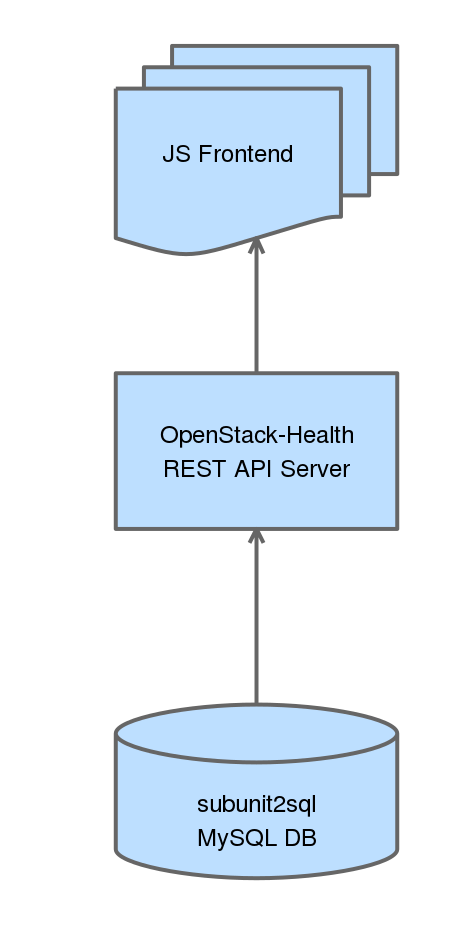
\includegraphics[height=1.2\textheight]{openstack-health-arch.png}
    \end{center}
\end{frame}

\begin{frame}
    \frametitle{Using OpenStack Health}
    \begin{center}
        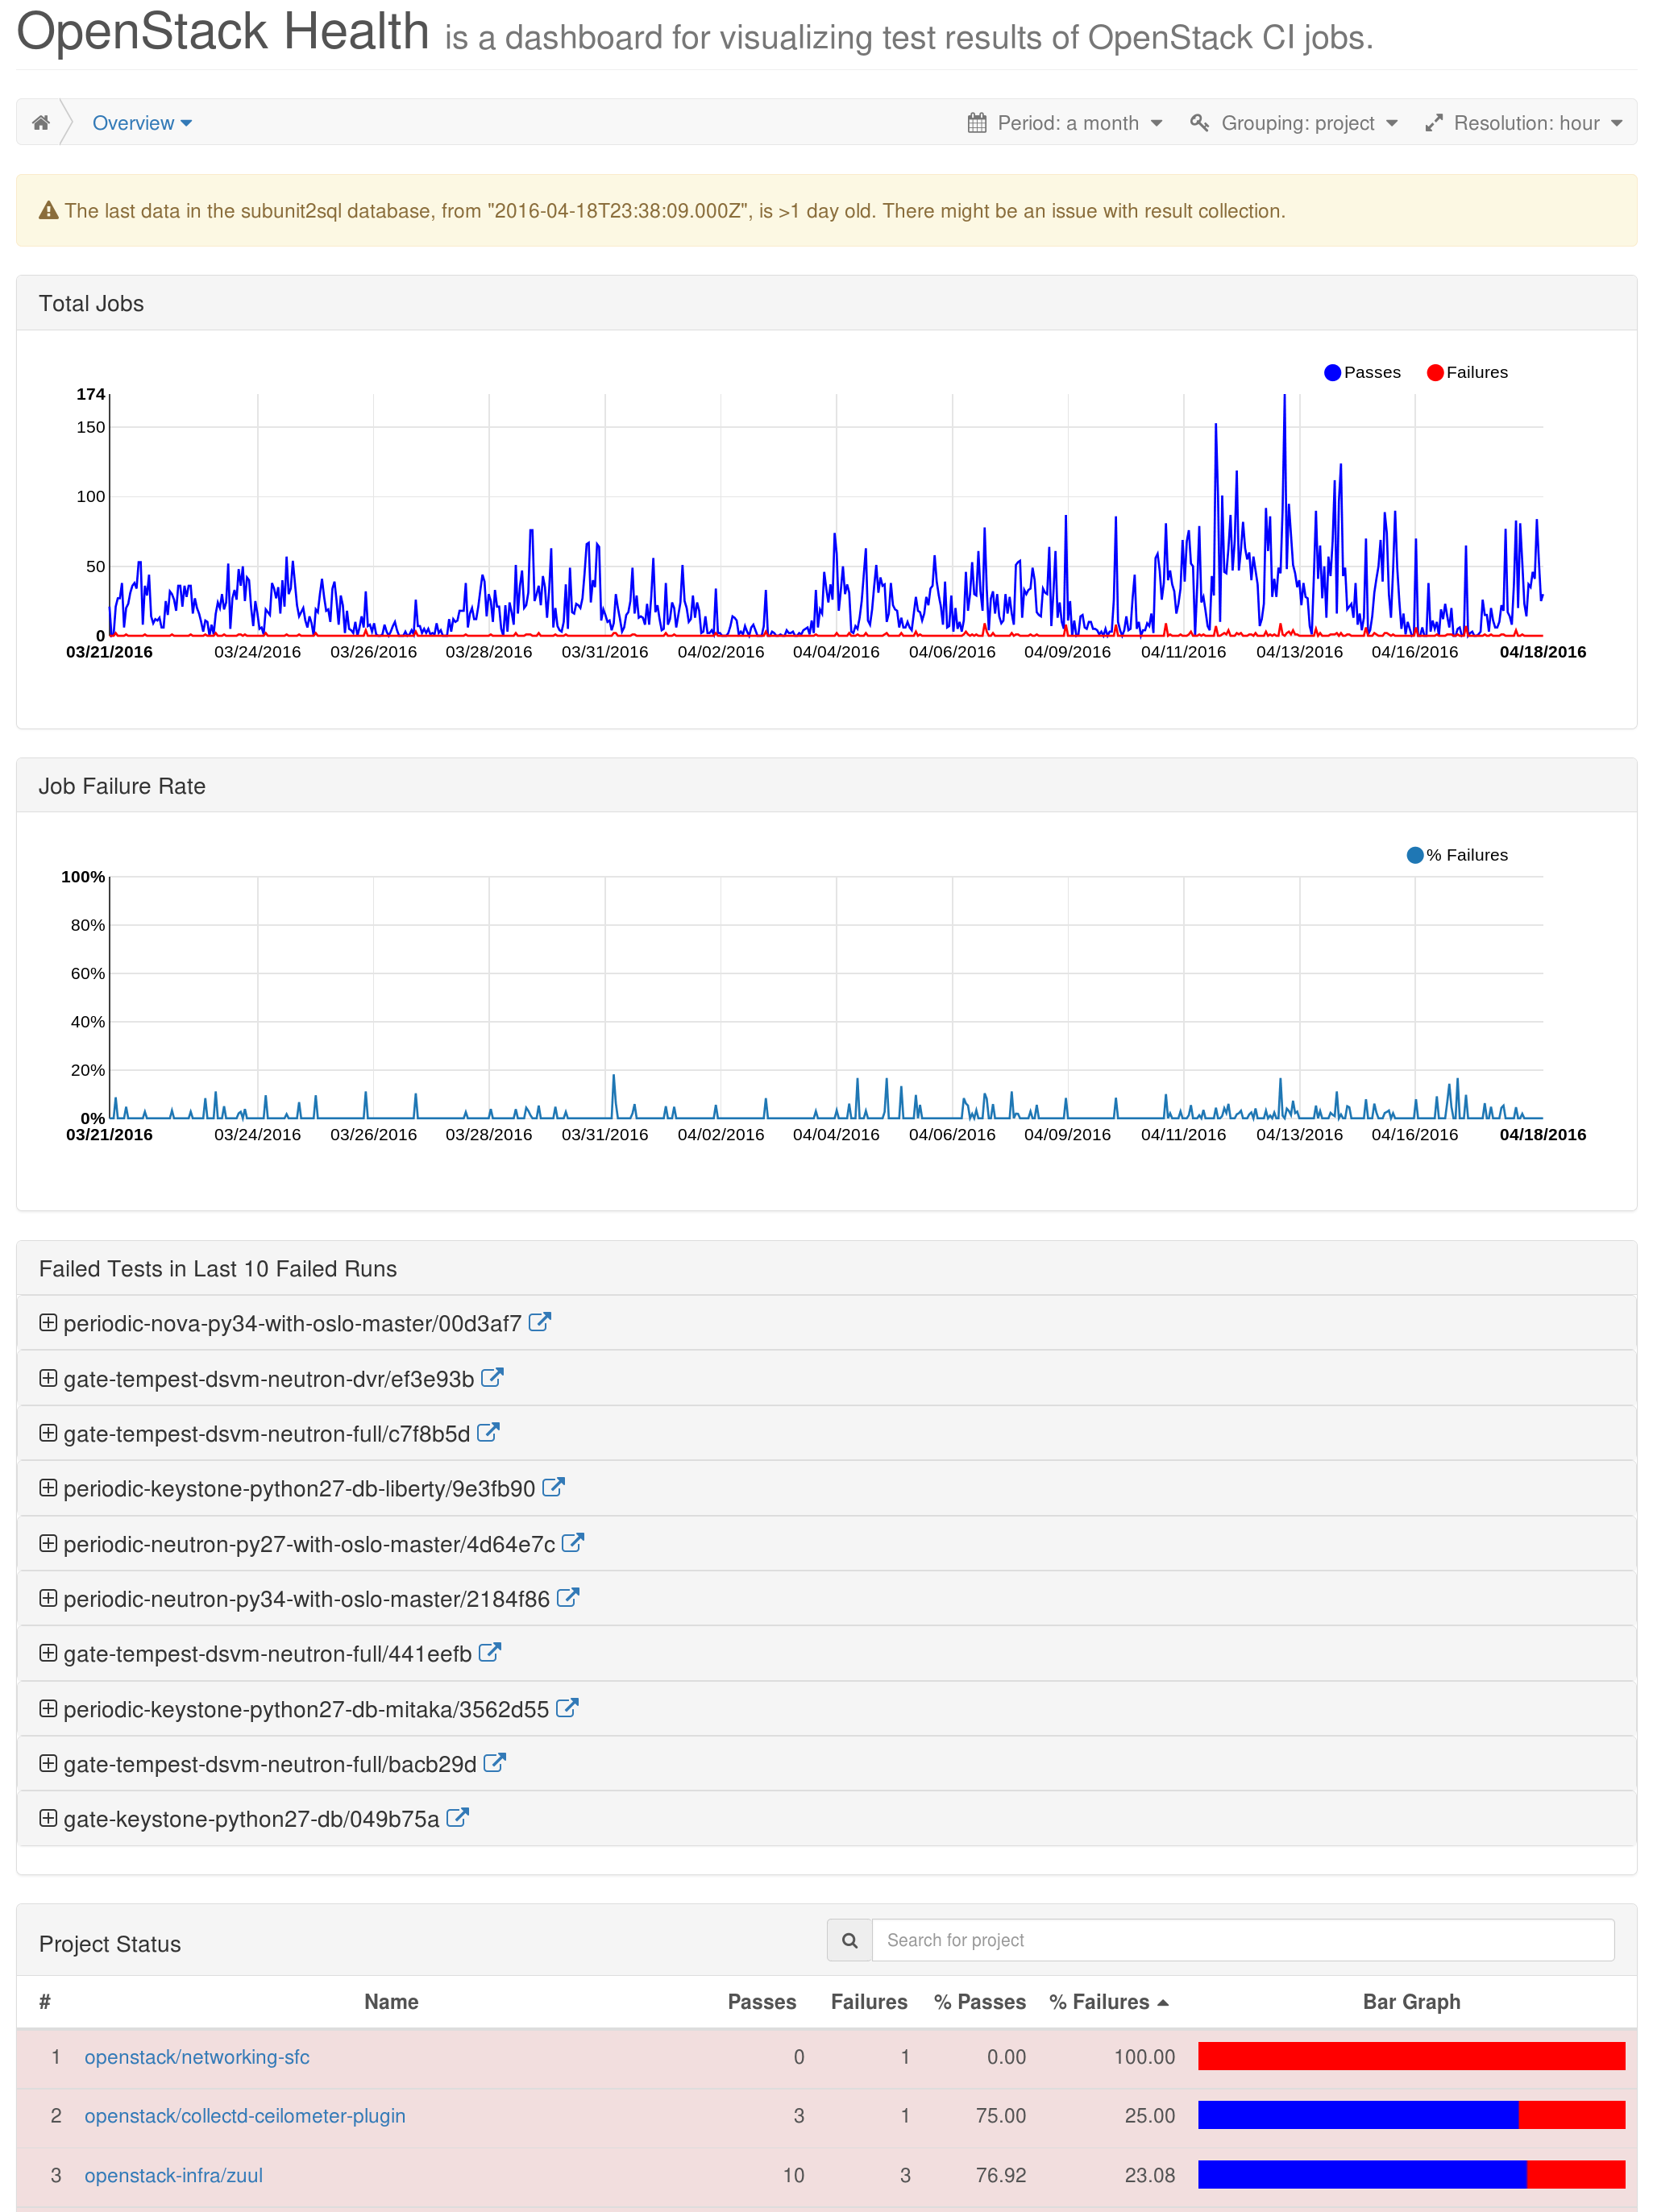
\includegraphics[height=.9\textheight]{HomePage.png}
    \end{center}
\end{frame}

\section{Results}
\begin{frame}
    \frametitle{Data Driven Decision Making}
    \begin{itemize}
        \item Determine when it's time to skip a test
        \item Identify tests that are actually catching bugs
        \item Determine if failures are isolated to region, config, etc.
        \item
    \end{itemize}
\end{frame}

\begin{frame}
    \frametitle{Finding trends amongst the noise}
    \begin{itemize}
        \item Catch performance regressions
        \item
    \end{itemize}
\end{frame}

\section{Future work/issues}

\begin{frame}
    \frametitle{Issues}
    \begin{itemize}
        \item Too many varied data sources each with unique limitations
        \item Only Gate and Periodic Job data (subunit2sql)
        \item No views for infra failure (subunit2sql)
        \item It'd difficult to get contribution from employees of companies
    \end{itemize}
\end{frame}

\begin{frame}
    \frametitle{Future work}
    \begin{itemize}
        \item Integrate all the things in openstack-health
        \item Use the data to optimize our test runner scheduler
        \item (Auto cause of failure detection with machine learning or something:)
    \end{itemize}
\end{frame}

\subsection{More Information}
\begin{frame}
\frametitle{Where to get more information}
    \begin{itemize}
        \item openstack-dev ML\: \href{mailto:openstack-dev@lists.openstack.org}{openstack-dev@lists.openstack.org}
        \item \#openstack-qa on Freenode
        \item \href{http://git.openstack.org/cgit/openstack/openstack-health/}{http://git.openstack.org/cgit/openstack/openstack-health/}
        \item \href{http://git.openstack.org/cgit/openstack-infra/subunit2sql}{http://git.openstack.org/cgit/openstack-infra/subunit2sql}
        \item \href{http://git.openstack.org/cgit/openstack-infra/elastic-recheck/}{http://git.openstack.org/cgit/openstack-infra/elastic-recheck/}
    \end{itemize}
\end{frame}

\section{Questions}
\begin{frame}
\frametitle{Questions?}
\end{frame}

\subsection{Appendix}
\begin{frame}
  \frametitle{Appendix: StackViz}
  Visualization tool of individual CI build results
  \begin{itemize}
    \item \href{http://git.openstack.org/cgit/openstack/stackviz}{git.openstack.org/cgit/openstack/stackviz}
  \end{itemize}
  \begin{center}
    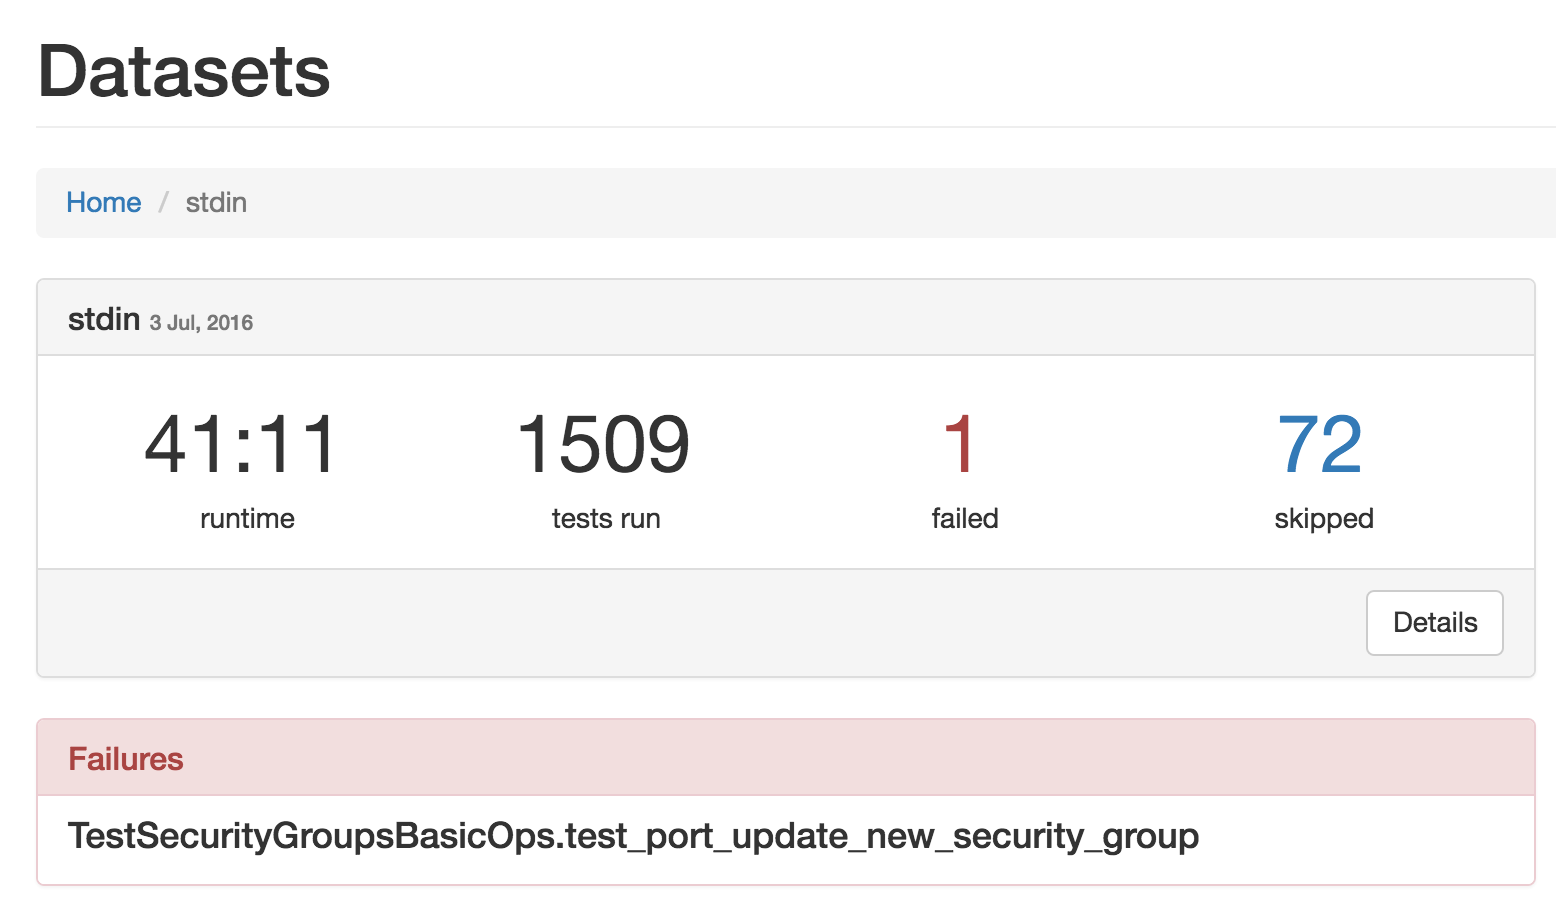
\includegraphics[width=1.3\textheight]{stackviz-sample-top.png}
  \end{center}
\end{frame}

\begin{frame}
  \begin{center}
    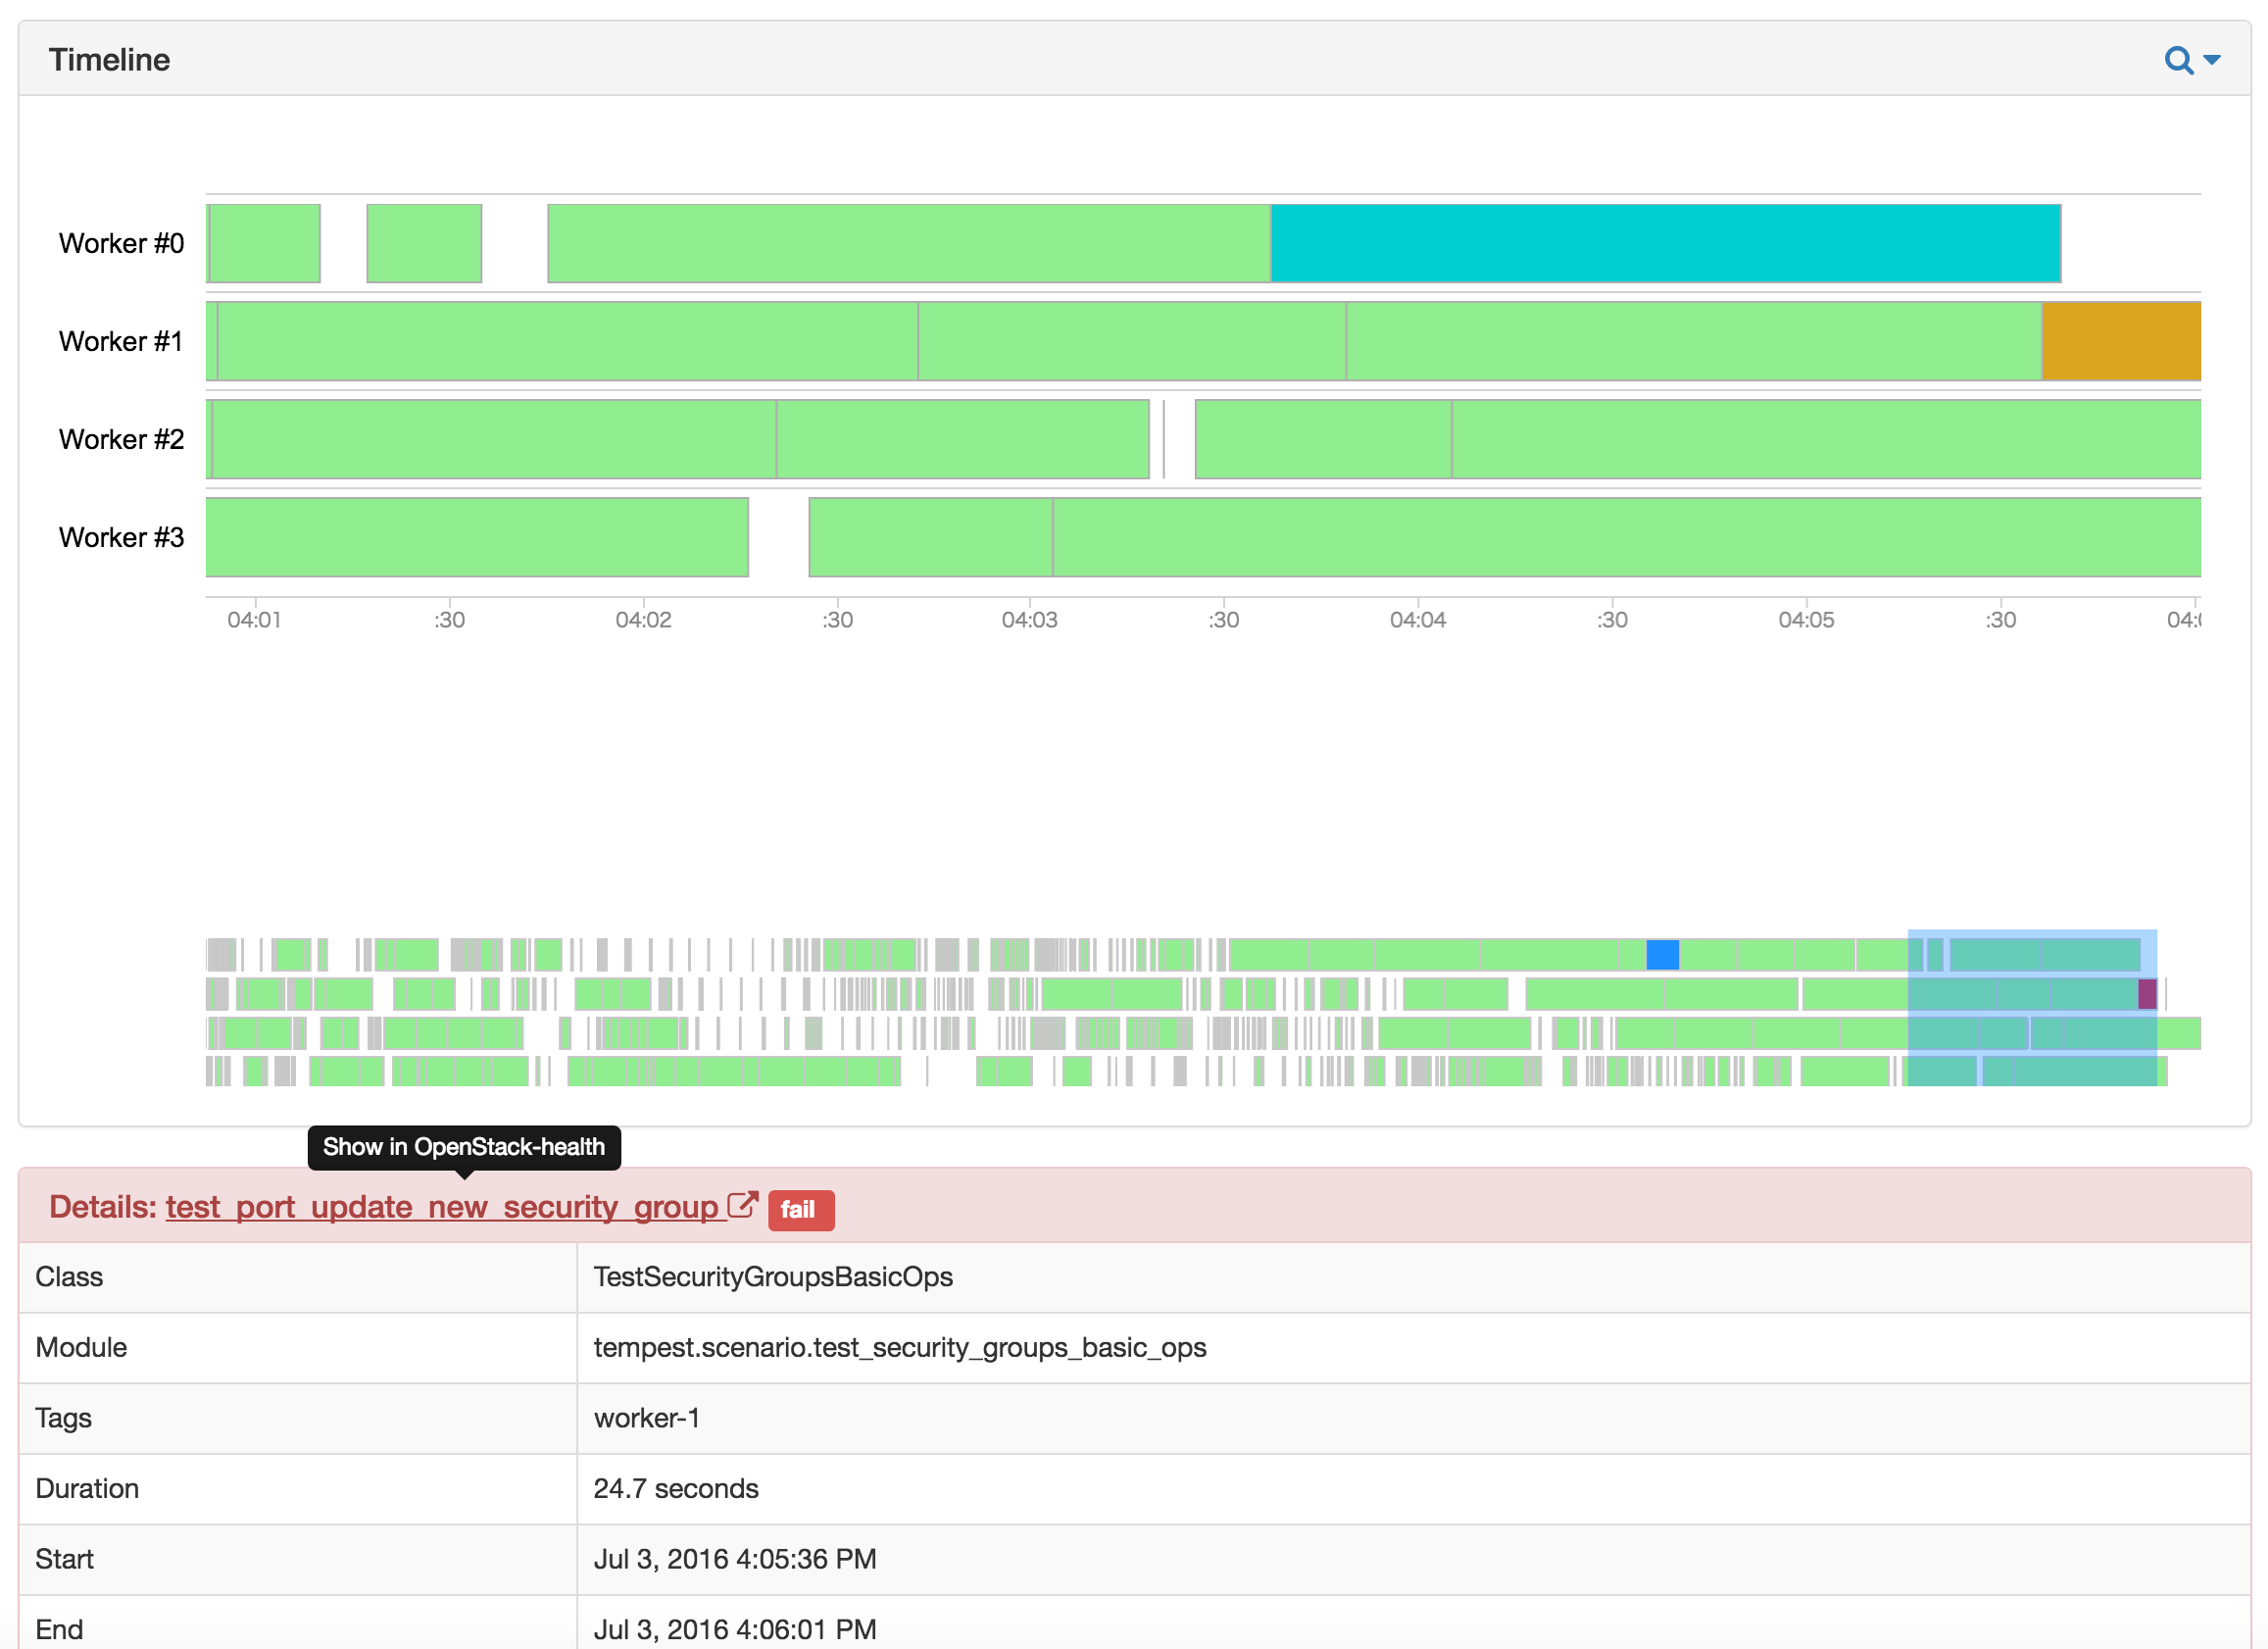
\includegraphics[width=1.3\textheight]{stackviz-sample-timeline.png}
  \end{center}
\end{frame}

\begin{frame}
  \begin{center}
    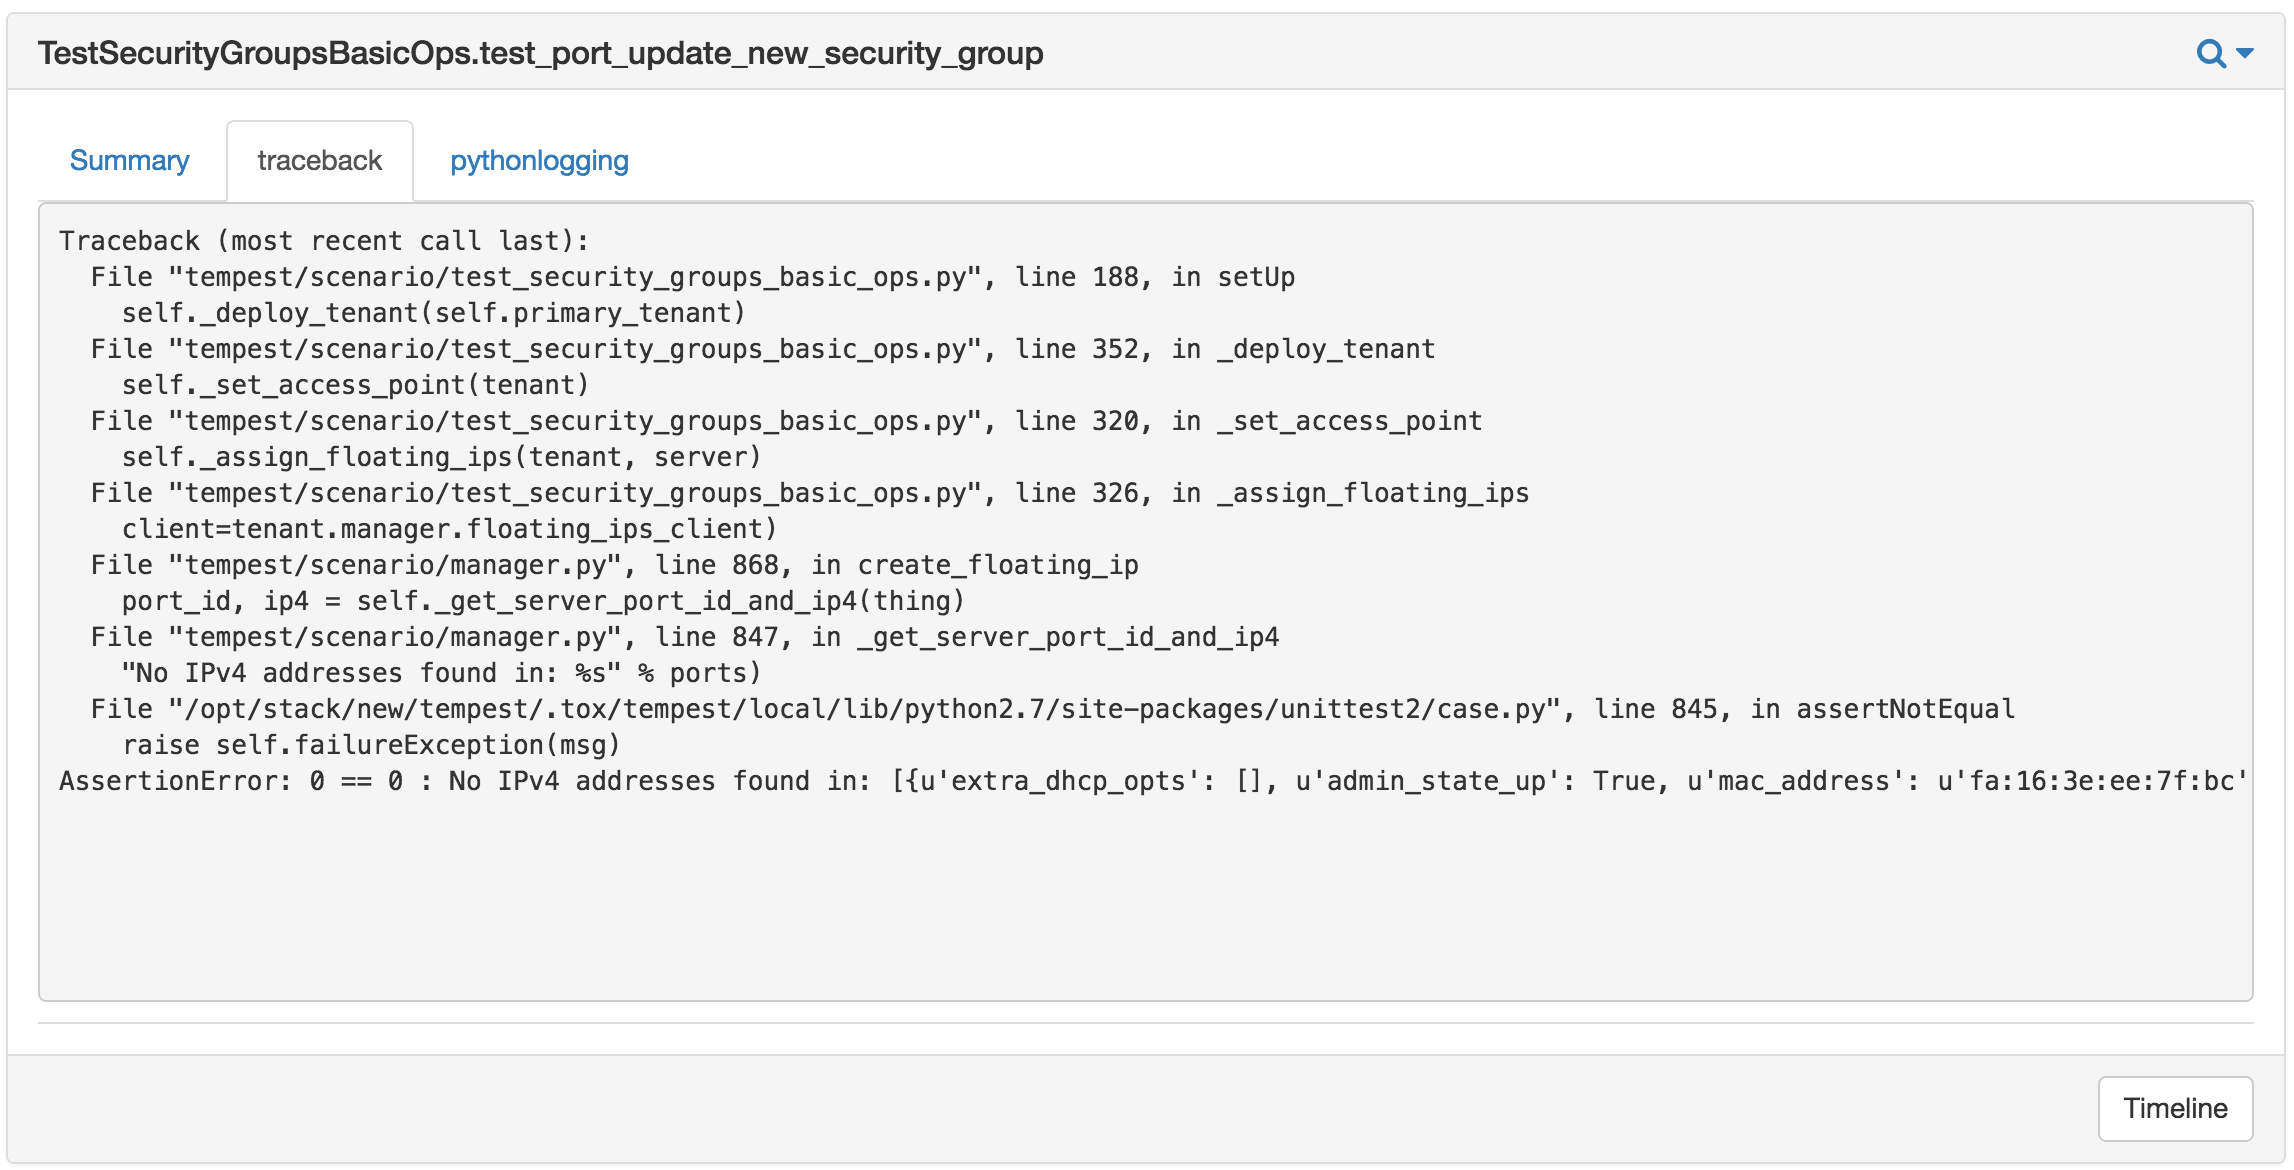
\includegraphics[width=1.3\textheight]{stackviz-sample-traceback.png}
  \end{center}
\end{frame}

\end{document}
